%%%%%%%%%%%%%%%%%%%%%%%%%%%%%%%%%%%%%%%%%%%%%%%%%%%%%%%%%%%%%%%%%%%%%%%%%%%%%%%%
%
% Template license:
% CC BY-NC-SA 3.0 (http://creativecommons.org/licenses/by-nc-sa/3.0/)
%
%%%%%%%%%%%%%%%%%%%%%%%%%%%%%%%%%%%%%%%%%%%%%%%%%%%%%%%%%%%%%%%%%%%%%%%%%%%%%%%%

%----------------------------------------------------------------------------------------
%	PACKAGES AND OTHER DOCUMENT CONFIGURATIONS
%----------------------------------------------------------------------------------------

\documentclass[
11pt, % The default document font size, options: 10pt, 11pt, 12pt
%oneside, % Two side (alternating margins) for binding by default, uncomment to switch to one side
%chapterinoneline,% Have the chapter title next to the number in one single line
spanish,
singlespacing, % Single line spacing, alternatives: onehalfspacing or doublespacing
%draft, % Uncomment to enable draft mode (no pictures, no links, overfull hboxes indicated)
%nolistspacing, % If the document is onehalfspacing or doublespacing, uncomment this to set spacing in lists to single
%liststotoc, % Uncomment to add the list of figures/tables/etc to the table of contents
%toctotoc, % Uncomment to add the main table of contents to the table of contents
parskip, % Uncomment to add space between paragraphs
%codirector, % Uncomment to add a codirector to the title page
headsepline, % Uncomment to get a line under the header
]{MastersDoctoralThesis} % The class file specifying the document structure



%----------------------------------------------------------------------------------------
%	INFORMACIÓN DE LA MEMORIA
%----------------------------------------------------------------------------------------

\thesistitle{Pantalla full color gigante} % El títulos de la memoria, se usa en la carátula y se puede usar el cualquier lugar del documento con el comando \ttitle

% Nombre del posgrado, se usa en la carátula y se puede usar el cualquier lugar del documento con el comando \degreename
\posgrado{Carrera de Especialización en Sistemas Embebidos} 


\author{Ing. Felipe Sarche} % Tu nombre, se usa en la carátula y se puede usar el cualquier lugar del documento con el comando \authorname

\director{Ing. Adrián Laiuppa (UTN-FRBB)} % El nombre del director, se usa en la carátula y se puede usar el cualquier lugar del documento con el comando \dirname
\codirector{Nombre del codirector (pertenencia)} % El nombre del codirector si lo hubiera, se usa en la carátula y se puede usar el cualquier lugar del documento con el comando \codirname.  Para activar este campo se debe descomentar la opción "codirector" en el comando \documentclass, línea 23.

\juradoUNO{Esp. Ing. Juan Vicente Montilla Cabrera (FIUBA)} % Nombre y pertenencia del un jurado se usa en la carátula y se puede usar el cualquier lugar del documento con el comando \jur1name
\juradoDOS{Dr. Ing. Pablo Martín Gomez (FIUBA)} % Nombre y pertenencia del un jurado se usa en la carátula y se puede usar el cualquier lugar del documento con el comando \jur2name
\juradoTRES{Dr. Ing. Ariel Lutenberg (FIUBA)} % Nombre y pertenencia del un jurado se usa en la carátula y se puede usar el cualquier lugar del documento con el comando \jur3name

%\ciudad{Ciudad Autónoma de Buenos Aires}
\ciudad{ciudad de Quito}

\fechaINICIO{marzo de 2020}
\fechaFINAL{diciembre de 2020}


\keywords{Sistemas embebidos, FIUBA} % Keywords for your thesis, print it elsewhere with \keywordnames


\begin{document}


\frontmatter % Use roman page numbering style (i, ii, iii, iv...) for the pre-content pages

\pagestyle{plain} % Default to the plain heading style until the thesis style is called for the body content


%----------------------------------------------------------------------------------------
%	RESUMEN - ABSTRACT 
%----------------------------------------------------------------------------------------

\begin{abstract}
\addchaptertocentry{\abstractname} % Add the abstract to the table of contents
%
%The Thesis Abstract is written here (and usually kept to just this page). The page is kept centered vertically so can expand into the blank space above the title too\ldots
\centering

En el presente documento se describe el diseño y la implementación de una pantalla fullcolor.Este sistema tiene como propósito informar a los conductores que transitan por los diferentes puntos de la ciudad datos útiles como por ejemplo tiempos de viaje, clima, mensajes de emergencia, etc.

Para la realización de este proyecto se integraron tres partes fundamentales software, hardware y verilog.
 


\end{abstract}

%----------------------------------------------------------------------------------------
%	CONTENIDO DE LA MEMORIA  - AGRADECIMIENTOS
%----------------------------------------------------------------------------------------

\begin{acknowledgements}
%\addchaptertocentry{\acknowledgementname} % Descomentando esta línea se puede agregar los agradecimientos al índice
\vspace{1.5cm}

A mi madre Ximena por apoyarme todo el tiempo. 
A Adrián Laiuppa, tutor de este trabajo por compartir su conocimiento.  
A mis compañeros de la Especialización en Sistemas Embebidos por sus paciencia y generosidad. 
A mis compañeros de trabajo por su ayuda.

\end{acknowledgements}

%----------------------------------------------------------------------------------------
%	LISTA DE CONTENIDOS/FIGURAS/TABLAS
%----------------------------------------------------------------------------------------

\tableofcontents % Prints the main table of contents

\listoffigures % Prints the list of figures

\listoftables % Prints the list of tables


%----------------------------------------------------------------------------------------
%	CONTENIDO DE LA MEMORIA  - DEDICATORIA
%----------------------------------------------------------------------------------------

\dedicatory{\textbf{Dedicado a... [OPCIONAL]}}  % escribir acá si se desea una dedicatoria

%----------------------------------------------------------------------------------------
%	CONTENIDO DE LA MEMORIA  - CAPÍTULOS
%----------------------------------------------------------------------------------------

\mainmatter % Begin numeric (1,2,3...) page numbering

\pagestyle{thesis} % Return the page headers back to the "thesis" style

% Incluir los capítulos como archivos separados desde la carpeta Chapters

% Chapter 1

\chapter{Introducción general} % Main chapter title

\label{Chapter1} % For referencing the chapter elsewhere, use \ref{Chapter1} 
\label{IntroGeneral}
En este capítulo se presentan los principales tipos de pantallas de mensajes variables, las características de las pantallas full color y por último se explica la motivación, el alcance y objetivos de este trabajo.
%----------------------------------------------------------------------------------------

% Define some commands to keep the formatting separated from the content 
\newcommand{\keyword}[1]{\textbf{#1}}
\newcommand{\tabhead}[1]{\textbf{#1}}
\newcommand{\code}[1]{\texttt{#1}}
\newcommand{\file}[1]{\texttt{\bfseries#1}}
\newcommand{\option}[1]{\texttt{\itshape#1}}
\newcommand{\grados}{$^{\circ}$}

%----------------------------------------------------------------------------------------

%\section{Introducción}

%----------------------------------------------------------------------------------------
\section{Pantallas de mensaje variable}

Los paneles de mensajes variables son señales de tránsito diseñadas para alertar o informar a los conductores. La pantalla de mensajes variables puede mostrar pictogramas o mensajes escritos. Las imágenes en pantalla pueden ser estáticas, parpadeantes o realizar efectos \cite{WIKIVMS}.


\subsection{Pantallas fijas}

Las pantallas fijas de mensajes variables generalmente se montan en estructuras aéreas que abarcan en voladizo una parte de la carretera, o fuera de la carretera, y se utilizan para influir en los conductores con propósitos de control de tránsito. Sus mensajes pueden cambiarse manual, mecánica o electromecánicamente para proporcionar a los automovilistas información sobre congestión del tráfico, accidentes de tráfico, operaciones de mantenimiento, condiciones climáticas adversas, condiciones de la carretera, eventos organizados u otras características de la carretera. Un beneficio de las pantallas fijas de mensaje variable es que pueden desplegar mensajes más detallados y permitir un adecuado tiempo de exposición  para que los automovilistas comprendan los mensajes antes de llegar a un punto de decisión. En la figura \ref{fig:vmsp} se muestra una pantalla fija de mensajes variables \citep{VMSTYPES}.



\subsection{Pantallas móviles}

Las pantallas móviles de mensajes variables suelen estar montadas en un remolque con paneles solares, son de fácil movimiento y pueden ser colocadas cerca de puntos de decisión donde el conductor puede realizar una acción como por ejemplo tomar un camino alterno o disminuir la velocidad. Sus mensajes se pueden cambiar de forma manual, mecánica o por medios electromecánicos. Un beneficio de los paneles de mensajes variables móviles es la posibilidad de ubicación en puntos estratégicos. En la figura \ref{fig:vmsm} se muestra una pantalla móvil de mensajes variables \citep{VMSTYPES}.

\begin{figure}[htpb]
	\centering
	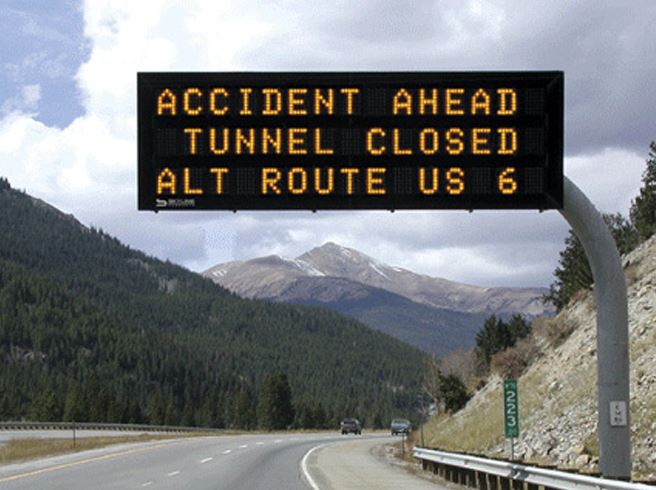
\includegraphics[width=.9 \textwidth]{../Figures/vmspermanente.jpg} 
	\caption{Pantalla fija \protect\footnotemark.}
	\label{fig:vmsp}
\end{figure}

\footnotetext{Imagen tomada de \url{https://www.skylineproducts.com/wp-content/uploads/2016/07/Walk-In.jpg}}

\begin{figure}[htpb]
	\centering
	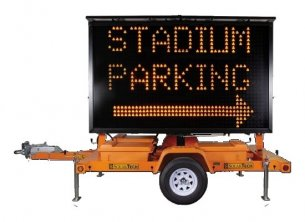
\includegraphics[width=.7\textwidth]{../Figures/vmsmovil.jpg} 
	\caption{Pantalla móvil \protect\footnotemark.}
	\label{fig:vmsm}
\end{figure}
\footnotetext{Imagen tomada de \url{https://www.enterpriseflasher.com/assets/images/solartech-1364402479.jpg}}

\pagebreak
\subsection{Pantallas montadas en camión}

Las pantallas de mensajes variables montadas en camión son generalmente unidades pequeñas ubicadas en o cerca de la parte trasera de un camión. Los paneles montados en camión generalmente tienen espacio reducido para mensajes y tamaños de fuente. Las limitaciones de sus mensajes suelen resultar en el uso de gráficos como flechas para facilitar la comprensión del conductor \citep{VMSTYPES}.

\begin{figure}[htpb]
	\centering
	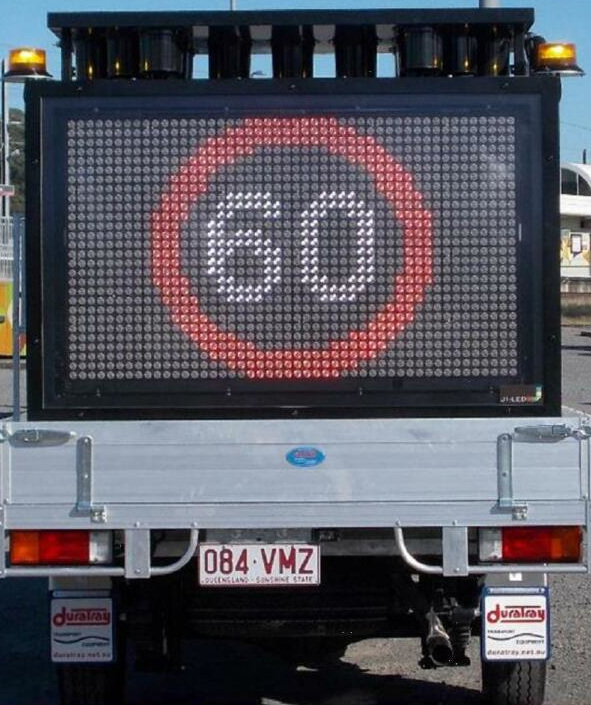
\includegraphics[scale=1]{../Figures/vmstruck.png} 
	\caption{Pantalla montada en camión \protect\footnotemark.}
	\label{fig:vmsc}
\end{figure}
\footnotetext{Imagen tomada de  \url{https://www.mobilesystems.co.nz/vdb/image/i2123}}


\section{Pantalla full color}
La pantalla de full color es un dispositivo electrónico compuesto por arreglos matriciales de LEDs. Dichos LEDs forman píxeles. Con los píxeles se puede formar textos, imágenes y hasta vídeo. Las pantallas LED se fabrican de una forma modular con el propósito de facilitar la instalación, transporte y mantenimiento. A continuación se enumeran algunas de las características de una pantalla full color \citep{WIKIPANTALLAFULLCOLOR}.


\subsection{Full color}
\textit{Full color} es un termino que significa que los colores primarios (rojo, verde y azul ) se mezclan para producir millones de tonos individuales. Para representar colores en pantallas se utiliza frecuentemente el modelo RGB en donde cada color es la suma de los colores rojo, verde y azul. Mediante la mezcla de estos tres colores con diferente intensidad se representan distintos colores.



\subsection{Resolución de pantalla}
La resolución de una pantalla se define como la cantidad de píxeles que esta posee. Se expresa como el producto de la cantidad de filas por el número de columnas \citep{WIKIRESOL}. Mientras mayor sea la resolución mayor cantidad de detalles se podrán apreciar en la imagen como se muestra en la figura \ref{fig:grafresolucion}.

\begin{figure}[htpb]
	\centering
	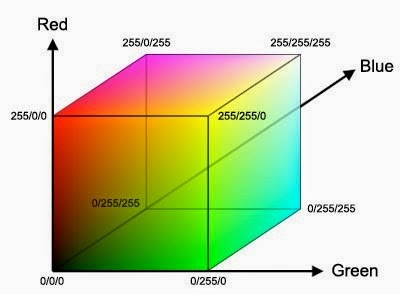
\includegraphics[scale=0.6]{Figures/modelorgb.jpg} 
	\caption{Modelo RGB\protect\footnotemark.}
	\label{fig:grafrgb}
\end{figure}
\footnotetext{Imagen tomada de \url{http://3.bp.blogspot.com/-NiYCndNGwHk/VCT\_ ywjC8FI/AAAAAAAAApk/0WDDtMziu6I/s1600/RGB1.jpg}}

\begin{figure}[htpb]
	\centering
	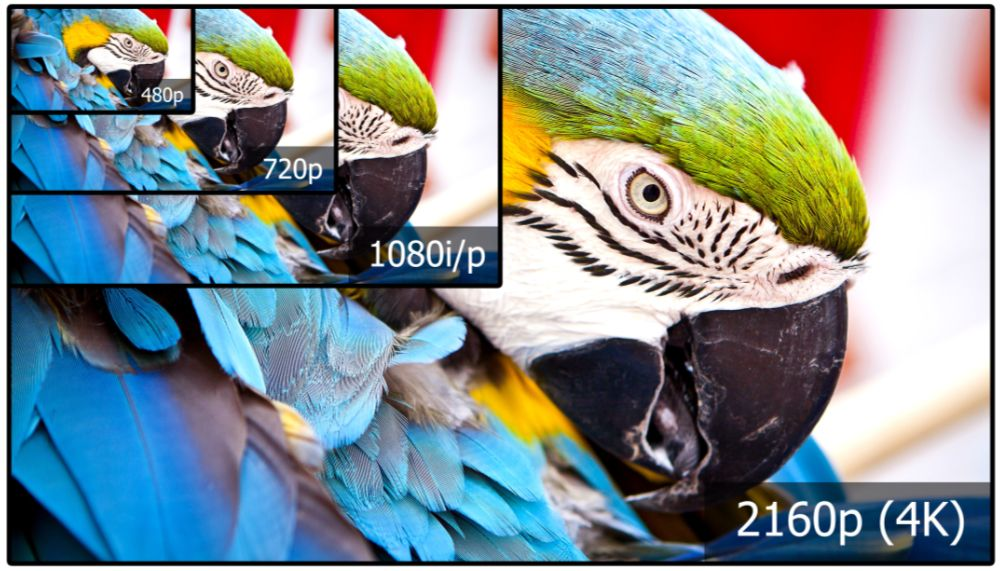
\includegraphics[scale=0.3]{Figures/resolucion.jpg} 
	\caption{Representación gráfica de resolución\protect\footnotemark.}
	\label{fig:grafresolucion}
\end{figure}
\footnotetext{Imagen tomada de \url{https://www.4kmonitor.net/wp-content/uploads/2020/03/4K-Monitor-Vor-und-Nachteile.jpg}}

\subsection{Píxel pitch}
Se define \textit{píxel pitch} a la distancia física que separa a los LEDs que conforman la pantalla. Esta distancia es medida en milímetros. La resolución de la pantalla tiene relación directa con el \textit{pitch}. Mientras más pequeño sea el \textit{pitch} mayor será la resolución para un mismo tamaño de pantalla \citep{IMAGENDEF2}. La figura \ref{fig:pixelpitch} muestra paneles LED en los que se resalta el \textit{pitch}.

Se suele abreviar esta medida con un "P-" seguida de la medida en milímetros. Por ejemplo la pantalla de esta memoria es una pantalla P-20.



\subsection{Tamaño de pantallas gigantes}
No existe ningún estándar para definir el tamaño de las pantallas gigantes. Las pantallas LED  se pueden construir uniendo módulos LED hasta alcanzar el tamaño deseado. La selección del \textit{pitch} de las pantalla gigantes para exteriores depende de la distancia del espectador como se puede observar en la figura \ref{fig:pitchview}.

\begin{figure}[htpb]
	\centering
	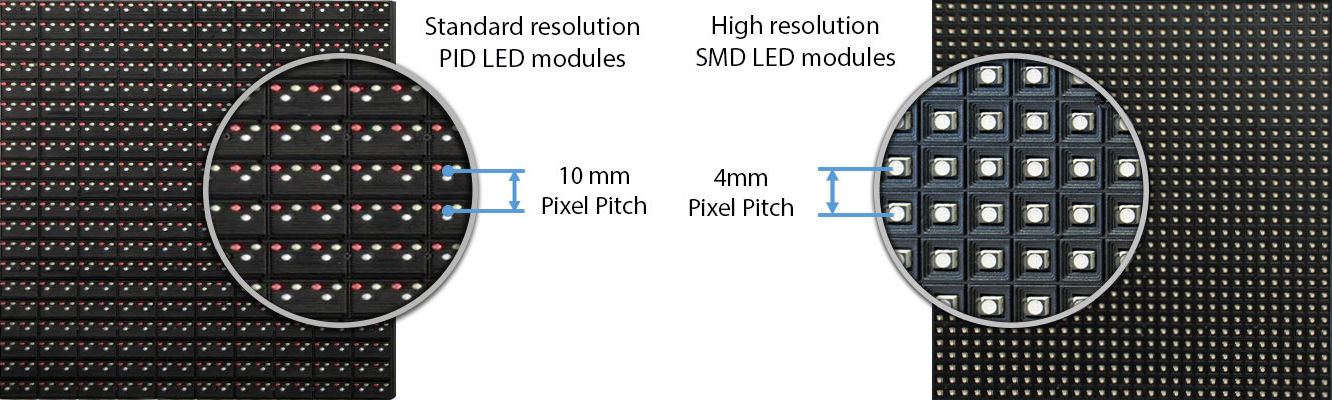
\includegraphics[scale=0.3]{Figures/pitch.jpg} 
	\caption{Representación gráfica de \textit{pitch}\protect\footnotemark.}
	\label{fig:pixelpitch}
\end{figure}
\footnotetext{Imagen tomada de \url{https://www.finepixelled.com/theme/basic-knowledge/pixel-pitch-resolution.jpg}}

\begin{figure}[htpb]
	\centering
	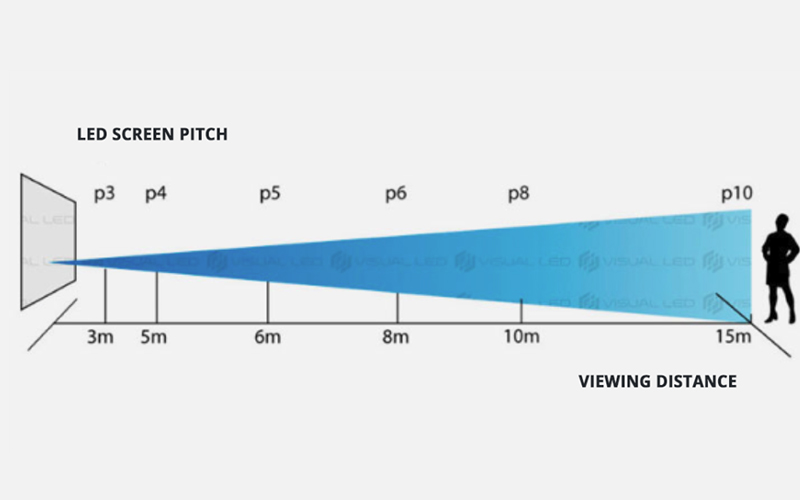
\includegraphics[scale=0.6]{Figures/visionpitch.jpg} 
	\caption{Selección de \textit{pitch} deacuerdo a la distancia del espectador \protect\footnotemark.}
	\label{fig:pitchview}
\end{figure}
\footnotetext{Imagen tomada de \url{https://www.doitvision.com/wp-content/uploads/2020/07/led-display-visual-distance.jpg}}


\subsection{Tasa de refresco}
La tasa de refresco se define como la frecuencia con la que la pantalla actualiza su imagen por cada segundo. La diferencia con respecto a FPS (Frames por segundo) es que esta magnitud también cuenta los fotogramas idénticos \citep{WIKITASA}.




\section{Paneles informativos comerciales}
Existe una gran cantidad de fabricantes de pantallas LED P-20 para exteriores. El país líder en producción de pantallas LED para exteriores es China. En la tabla \ref{tab:comercial} se muestra una comparación de las características de algunas pantallas comerciales. De esta comparación se puede observar que las pantallas comerciales comparten características muy similares a excepción de el consumo de energía. El consumo de energía esta relacionado con el tipo de LED que se usa para construir la pantalla. 

\begin{table}[h]
\centering
\caption[Comparación entre pantallas P-20]{Comparación de características de pantallas P-20 comerciales.}
\begin{tabular}{l c c c}
\toprule
\textbf{Característica} & \textbf{S. Chuangkaiguang Co \citep{TABLAREF1}} & \textbf{Leeman \citep{TABLAREF2}} & \textbf{Samsung \citep{TABLAREF3}} \\
\midrule 

Ángulo de visión        & H120,V60 & H 120,V 60 & H140,V 59 \\
Constitución de píxel   & RGB & RGB & RGB \\
Tasa de refresco        & mayor a 60 Hz & 60 Hz & 60 Hz \\
Consumo promedio        & \SI{200}{\watt\per\meter\squared} & \SI{200}{\watt\per\meter\squared} & \SI{169}{\watt\per\meter\squared} \\
Grado de protección     & IP65 & IP65 & IP65 \\

\bottomrule
\hline
\end{tabular}
\label{tab:comercial}
\end{table}





\section{Motivación}
Existieron muchos motivos que llevaron a la creación de una pantalla full color gigante. El motivo principal fue la necesidad de desarrollar y construir productos de alto valor agregado de manera local. Dentro de Ecuador no existe ninguna empresa que construya pantallas gigantes. Existen muchas empresas dedicadas a comercializar pantallas importadas. 

Otro de los motivos es que en Ecuador los impuestos de importación a productos terminados es muy alto. Construir la pantalla en el país es una opción viable gracias a estos impuestos. El tercer motivo es la representación local del producto, ya que la empresa se encuentra dentro del país puede garantizar el servicio técnico durante el tiempo del contrato. Finalmente desarrollar una pantalla LED full color fue un reto personal que forma parte de mi desarrollo profesional. 



\section{Propósito del trabajo}
El propósito de este trabajo fue desarrollar una pantalla gigante full color LED. Se espera que el desarrollo de este nuevo producto diversifique el portafolio de productos viales que ya posee la empresa.

\pagebreak
\section{Alcance del trabajo}
El presente proyecto incluye:

\begin{itemize}
\item Diseño y construcción de una pantalla LED de 384 por 96 píxeles.
\item Manuales de ensamblaje eléctrico de la pantalla.
\item Desarrollo de firmware de la pantalla.
%\footnotetext{Referencia de placa  https://www.terasic.com.tw/cgi-bin/page/archive.pl?Language=English\&No=836}


\end{itemize}

El presente proyecto no incluye:

 \begin{itemize}
\item La interfaz gráfica para el cargado remoto de la imágenes.
\item La aplicación para cargar imágenes en forma local.
\item Diseño de ventilación 
\item Diseño de mecánica de armado.

\end{itemize}





\chapter{Introducción específica} % Main chapter title

\label{Chapter2}

%----------------------------------------------------------------------------------------
%	SECTION 1
%----------------------------------------------------------------------------------------
Este capítulo explica las tecnologías aplicadas en el desarrollo de la pantalla gigante full color. Se presentan los requerimientos identificados al iniciar el trabajo para cumplir con los objetivos.
\section{Matriz de LEDs}
La matriz de LEDs es un conjunto o arreglo de LEDs  bidimensional donde los cátodos se unen en filas y los ánodos se unen en columnas. Existen numerosos métodos para controlar las matrices de LEDs. Para desarrollar este proyecto se seleccionó el método de multiplexación debido a su bajo uso de recursos en comparación a controlar los LEDs de manera individual \citep{CONCEPTOMATRIZ}.
\subsection{Multiplexación de una Matriz de LEDs }
La multiplexación es una técnica de control de matrices LED en donde se habilita de forma secuencial una fila de LEDs a la vez y las columnas se habilitan de acuerdo a la imagen que se desea mostrar en la matriz de LEDs. Una vez terminado el proceso para todas las filas de LEDs se procede a comenzar el ciclo nuevamente. La frecuencia del ciclo debe ser superior a 30 Hz para evitar que ojo humano detecte el parpadeo \citep{MULTIPLEXADO}.

En la figura \ref{fig:matrizled} se puede observar una matriz de LEDs de cuatro filas por cuatro columnas. Para mostrar la imagen se siguen los siguientes pasos:

\begin{enumerate}
\item Se habilita la fila T3.
\item Se habilita la columna N1.
\item Se espera un momento.
\item Se deshabilita la fila T3.
\item Se habilita la fila T2.
\item Se habilita las columnas N1, N2 y N3.
\item Se espera un momento.
\item Se deshabilita la fila T2.
\item Se habilita la fila T1.
\item No se habilita ninguna columna.
\item Se espera un momento.
\item Se deshabilita la fila T1.
\item Se habilita la fila T0.
\item No se habilita ninguna columna.
\item Se espera un momento.
\item Se deshabilita la fila T0.
\item Se repite el ciclo desde el paso uno.
\end{enumerate}


\begin{figure}[htpb]
	\centering
	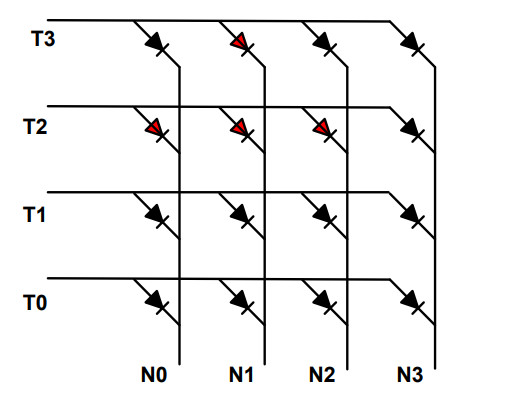
\includegraphics[scale=0.5]{Figures/ledmatrix.jpg} 
	\caption{Matriz de LEDs \protect\footnotemark.}
	\label{fig:matrizled}
\end{figure}

\footnotetext{Imagen tomada de \url{https://web.stanford.edu/class/archive/engr/engr40m.1178/slides_sp17/lecture10.pdf}}

Una de las maneras de habilitar las filas es a través de MOSFET canal P y las columnas se habilitan a través de drivers de LEDs \citep{CONCEPTOMATRIZ}.
 
 

%\https://bibdigital.epn.edu.ec/bitstream/15000/9935/1/SISTEMA%20DE%20INFORMACION%20VISUAL.pdf




\subsection{Driver de LED MBI5051}
El driver que se eligió para habilitar las columnas de LEDs fue el driver MBI5051. Este driver es un producto de la empresa MACROBLOCK. En diseños anteriores se usaron drivers de esta empresa. Este driver fue diseñado para ser usado en pantallas exteriores de vídeo. Las características del driver se muestran en la tabla \ref{tab:driverled}. 

\begin{table}[h]
\centering
\caption[Características MBI5051]{Características del driver MBI5051 \protect\footnotemark.}
\begin{tabular}{l c c}
\toprule
\textbf{Especificaciones}& \textbf{Detalles}\\
\midrule 

Voltaje alimentación & 3,0 V-5,5 V\\
Canales de corriente constante & 16\\
Rango de corriente constante por canal & 2 a 45 mA\\
Profundidad de color & 14 o 16 bits\\
Máxima frecuencia de reloj & 30 MHz\\

\bottomrule
\hline
\end{tabular}
\label{tab:driverled}
\end{table}

\footnotetext{Referencia tomada de \url{https://www.neumueller.com/datenblatt/macroblock/MBI5051\%20Datenblatt\%20-\%20Datasheet.pdf}}

\section{LED SMD CLX6F}
Los principales productores de LEDs son CREE ,EPISTAR ,NICHIA ,SEOUL SEMICONDUCTOR, Toyoda Gosei y Agilent.
El LED que fue elegido para la construcción de la pantalla fue el LED SMD CLX6F. El LED SMD CLX6F forma parte del catálogo de productos de la empresa CREE. Se logró contactar con una empresa en Shenzhen que usaba el \textit{chip} de CREE pero agregaba un encapsulado propio, lo que abarato el precio del LED. Este es un LED tricolor diseñado para ser usado en pantallas exteriores de vídeo. Las características principales del LED son:
\begin{itemize}
\item Resistencia al agua IPX8.
\item Luminosidad del rojo 560 mcd a 1120 mcd.
\item Luminosidad del verde 900 mcd a 1800 mcd.
\item Luminosidad del azul 140 mcd a 355 mcd.
\item El encapsulado del LED contiene inhibidores de UV lo cual minimiza el efecto a largo plazo de los rayos solares.
\end{itemize}

Las características eléctricas máximas se muestra en la tabla \ref{tab:MAXLEDCLX6F}.


\begin{table}[h]
\centering
\caption[Características eléctricas máximas LED CLX6F]{Características eléctricas máximas LED SMD CLX6F \protect\footnotemark.}
\begin{tabular}{l c c c c}
\toprule
\textbf{Especificaciones}& \textbf{R} & \textbf{G} & \textbf{B}\\
\midrule 


Corriente directa &50 mA &35 mA &35 mA\\
Corriente directa pico &200 mA &100 mA &100 mA \\
Voltaje inverso &5 V &5 V &5 V\\
Temperatura de operación &-40\si{\degree} C a 100\si{\degree} C  &-40\si{\degree} C a 100\si{\degree} C  &-40\si{\degree} C a 100\si{\degree} C\\


\bottomrule
\hline
\end{tabular}
\label{tab:MAXLEDCLX6F}
\end{table}

\footnotetext{Referencia tomada de \url{https://cree-led.com/media/documents/ds-CLX6F-FKC-1352.pdf}}



\section{ Plataforma de desarrollo DE1SoC}
Para la realización del trabajo se utilizó la plataforma de desarrollo DE1SoC debido a que cumple con los requerimientos y a que la empresa la usó en el desarrollo de proyectos previos. Esto último ahorró mucho tiempo de aprendizaje. Las especificaciones de la plataforma se muestran en la tabla \ref{tab:DE1SOCTABLA}.

\begin{table}[h]
\centering
\caption[Especificaciones DE1SoC]{Especificaciones DE1SoC \protect\footnotemark.}
\begin{tabular}{l c c}
\toprule
\textbf{Especificaciones}& \textbf{Detalles}\\
\midrule 


Procesador & ARM CORTEX A9\\
HPS SDRAM & 1GB DDR3\\
FPGA SDRAM & 64MB SDRAM\\
UART & UART a USB\\
FLASH & EPCS128\\
Puertos USB & 2\\
Pines GPIO & 36x2\\
Ethernet & 1 Gigabit\\


\bottomrule
\hline
\end{tabular}
\label{tab:DE1SOCTABLA}
\end{table}

\footnotetext{Referencia tomada de \url{https://www.terasic.com.tw/cgi-bin/page/archive.pl?Language=English&CategoryNo=205&No=836&PartNo=1}}

La plataforma cuenta con un procesador y un FPGA dentro del mismo \textit{chip} como se puede observar en la figura  \ref{fig:DE1BLOCK}. El FPGA fue usado para controlar la matriz de LEDs debido a su capacidad de manejar varias salidas GPIO en paralelo. Mientras que el procesador fue usado para manejar las comunicaciones.

\begin{figure}[htpb]
	\centering
	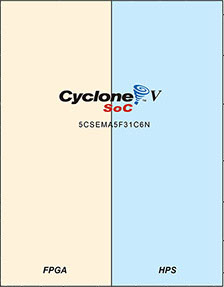
\includegraphics[scale=0.7]{Figures/fpgablock.jpg}  
	\caption{Diagrama de bloques DE1-SoC \protect\footnotemark.}
	\label{fig:DE1BLOCK}
\end{figure}

\footnotetext{Referencia tomada de \url{https://www.terasic.com.tw/attachment/archive/836/image/image_77_thumb.jpg}}


\section{Lenguaje descriptor de hardware}


El lenguaje seleccionado para describir el hardware fue \textit{verilog}. El lenguaje posee un preprocesador similar al lenguaje C, ademas de compartir palabras reservadas de control. A pesar de tener una sintaxis muy similar a C difiere en la definición de constantes, requiere la longitud de bits, no tiene estructuras, apuntadores o funciones recursivas. 

En verilog no todas las sentencias del lenguaje son sintetizables. Si las sentencias de todos los módulos son sintetizables, se pueden convertir en una lista de nodos que describe los componentes básicos. ``La lista de nodos puede entonces ser transformada en una forma describiendo las celdas estándar de un circuito integrado, por ejemplo ASIC, o una cadena de bits para un dispositivo de lógica programable (PLD) como puede ser una FPGA o un CPLD'' \citep{WIKIVERILOG}.




\section{Protocolo de comunicaciones UDP}
UDP es el acrónimo de protocolo de datagrama de usuario. UDP es un protocolo de comunicaciones que pertenece a la capa de transporte. Este protocolo permite la transmisión de datos sin conexión preliminar y no define la confirmación de recepción. Se usa en aplicaciones en donde el intercambio de paquetes de la conexión o desconexión son mayores a la información transmitida o en aplicaciones de transmisión de audio y vídeo en tiempo real debido a que retransmitir agregaría retardos \citep{WIKIUDP}.


\section{Sistema operativo de propósito general para embebidos}

El sistema operativo que se utilizó en el desarrollo de este trabajo fue Linux embebido. Linux embebido se refiere al uso del núcleo Linux  en un sistema embebido combinado con un conjunto de utilidades de software libre. 
%\https://es.wikipedia.org/wiki/Linux_embebido
El núcleo de Linux o \textit{kernel} es la interfaz entre el hardware de un PC y sus procesos \citep{KERNEL}. Las tareas que realiza el \textit{kernel} son:

\begin{itemize}
\item Gestión de memoria: control de cantidad de memoria y locación de la misma.
\item Gestión de procesos: administra que procesos usan la CPU y cuanto tiempo.
\item Controladores de dispositivos: interfaz entre hardware y procesos.
\item Seguridad y llamadas de sistema: recibe solicitud de servicio desde procesos. 
\end{itemize}


\subsection{SAMBA}
SAMBA es una aplicación que permite que las carpetas compartidas dentro del sistema operativo Linux, Mac OS X o Unix  puedan ser abiertas desde un computador con sistema operativo Windows \citep{WIKISAMBA}.

\subsection{Servicio de Linux}

Los servicios son programas que se ejecutan fuera de la vista y control del usuario ya que no cuentan con interfaz gráfica. Existe algunos servicios que son muy importantes para el funcionamiento del sistema operativo.
En sistemas UNIX o Linux, los servicios son conocidos como demonios \citep{SERVICIO}.

\subsection{SYSTEMD}

SYSTEMD es un software de administración de sistemas y servicios, el objetivo principal de este software es que la configuración y comportamiento de los servicios sea el mismo en todas las distribuciones de Linux. Se puede utilizar SYSTEMD para realizar configuraciones al iniciar el sistema \citep{REFSYSTEMD}.

\subsection{BASH script}
BASH es un interprete de comandos. Está presente en una amplia variedad de sistemas operativos y es el interprete de comandos por defecto en los sistemas Linux \citep{BASH}. 


BASH SCRIPT es un texto plano que contiene una serie de comandos. Esta lista de comandos es una mezcla de comandos que son comúnmente escritos por medio de la consola \citep{BASHSCRIPT}. El uso de bash scripting permite:

\begin{itemize}
\item Automatizar acciones repetitivas.
\item Mejor experiencia de usuario debido a lo anterior.
\item Ofrece herramientas al administrador para que el sistema operativo sea más ágil y automático.
\end{itemize}

\section{Requerimientos}
En esta sección se indican los requerimientos que fueron propuestos para el proyecto.

\subsection{Grupos de requerimientos asociados con hardware}

Tarjeta de distribución:
\begin{itemize}
\item Debe tener conectores de entrada IDC40 con la misma distribución de pines usados en las salidas GPIO de la board DE1-SoC.
\item Debe cambiar los niveles de voltaje de 3.3 v a 5 v de todas las entradas. 
\item Debe manejar señales de una frecuencia de entre 5 MHz a 10 MHz.
\item Debe tener conectores de salida IDC16 compatibles con la distribución de pines usados en las matrices de LEDs.
\end{itemize}
Matriz de LEDs:
\begin{itemize}
\item Debe tener un conector de entrada y un conector de salida IDC16.
\item Debe ser capaz de manejar frecuencias de hasta 10 MHz.
\item Debe tener drivers de LEDs con escala de grises de 16 bits.
\item Debe tener 16 LEDs de alto por 16 LEDs de ancho.
\item Debe ser capaz de pasar la información de la entrada a la salida.
\item Debe poder realizarse control por barrido. 
\item La pantalla tendrá una dimensión de 400 pixeles de largo por 96 pixeles máximo.
\end{itemize}

\subsection{Grupos de requerimientos asociados con el software}

Sistema operativo:
\begin{itemize}
\item Debe ser capaz de inicial y restablecer el programa del procesador automáticamente.
\item Debe ser capaz de conectarse a la red LAN. 
\item Debe ser capaz de compartir una carpeta para el proceso de cargado de imágenes.
\item Almacenamiento interno de hasta 500 imágenes.
\end{itemize}

Firmware procesador:
\begin{itemize}
\item Debe ser capaz de leer las imágenes que se encuentran en la carpeta compartida.
\item Debe ser capaz de escribir en una  memoria ram accesible para el FPGA  las imágenes a ser desplegadas.
\item Debe administrar el despliegue de las imágenes por medio de un archivo externo que sea enviado desde la central de control.
\end{itemize}
\subsection{Grupos de requerimientos asociados al FPGA}
FPGA:
\begin{itemize}
\item El FPGA debe ser capaz de manejar a la pantalla LED a una frecuencia de  30 hz.
\item Debe leer la información del los LEDs de una memoria ram que comparta con el procesador.
\item Debe manejar los drivers de LED a través de una máquina de estado finita.   
\end{itemize} 
\chapter{Diseño e implementación} % Main chapter title

\label{Chapter3} 
En este capítulo se realiza una explicación de la solución propuesta , el diseño de los circuitos impresos, el diseño del firmware y el diseño de la lógica programable.

\section{ Arquitectura de la solución propuesta}
Para cumplir los requerimientos enumerados en el capítulo \ref{Chapter2} se desarrollo la solución mostrada en la figura \ref{fig:solución}. Se utilizó la BOARD DE1-SoC en la cual se utilizó el FPGA para controlar la matriz de LEDs y el procesador para administrar el despliegue de las imagenes y manejar las comunicaciones con la estación remota.
\begin{figure}[htpb]
	\centering
	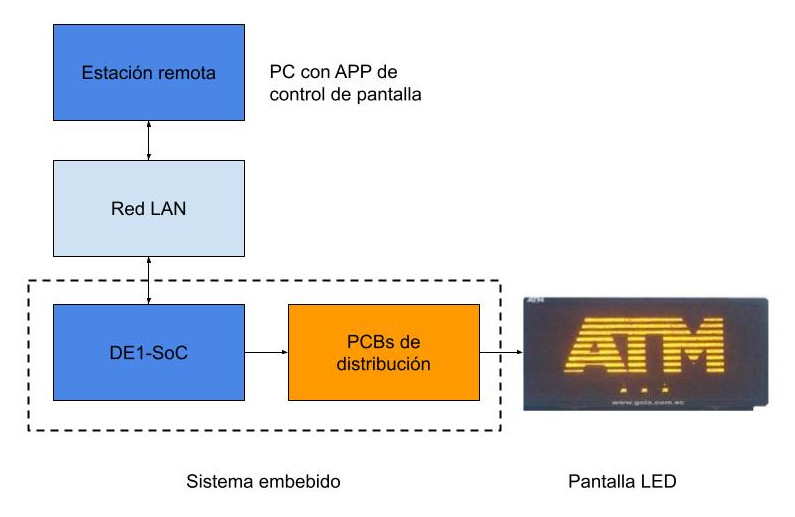
\includegraphics[scale=2]{Figures/Diagramasistemavms.jpg} 
	\caption{Esquema de la solución propuesta.}
	\label{fig:solución}
\end{figure}

En la figura \ref{fig:bloques embebido} se muestra el diagrama de bloques del sistema embebido. En la figura \ref{fig:bloques embebido} se muestra la interacción interna y externa de la BOARD DE1-SoC.
 
\begin{figure}[htpb]
	\centering
	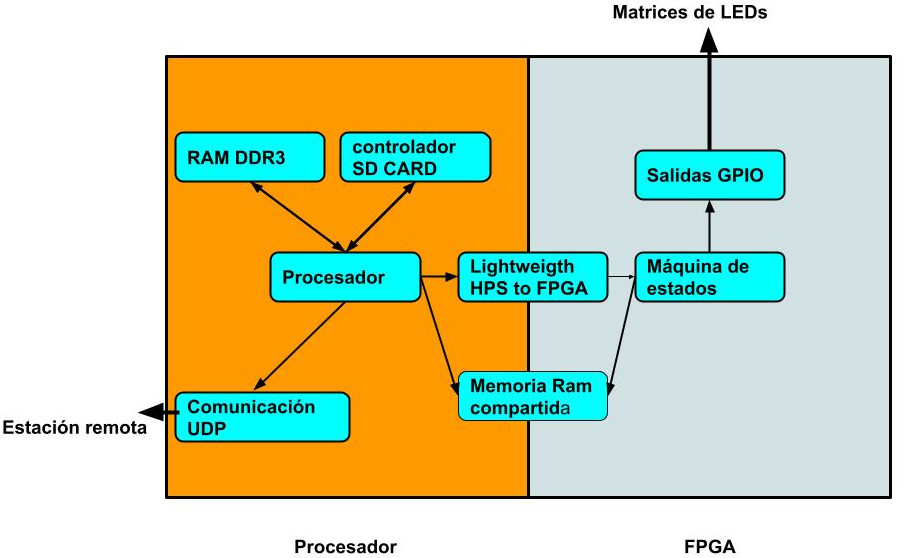
\includegraphics[scale=2]{Figures/Diagramabloques.jpg} 
	\caption{Diagrama de bloques del sistema embebido.}
	\label{fig:bloques embebido}
\end{figure}






\section{ Diseño de circuitos impresos}
Se diseñaron dos PCBs para la construcción de la pantalla, una PCB matriz de LEDs y una PCB para distribuir señales de control desde el FPGA hacia las matrices de LEDs.
\subsection{PCB matriz de LEDs}
Para construir la pantalla LED se utilizaron varias PCBs matrices de LEDs. La PCB matriz LEDs tiene una resolución de 16 LEDs de ancho por 16 LEDS de largo. Los LED tienen un \textit{pitch} P-20. Se utilizó el conector IDC-16 para recibir y transmitir las señales de control. En la figura \ref{fig:pcbrenderfront}  se muestra la PCB desde una perspectiva frontal. En la figura \ref{fig:pcbrenderback} se muestra el lado posterior de la PCB.


\begin{figure}[htpb]
	\centering
	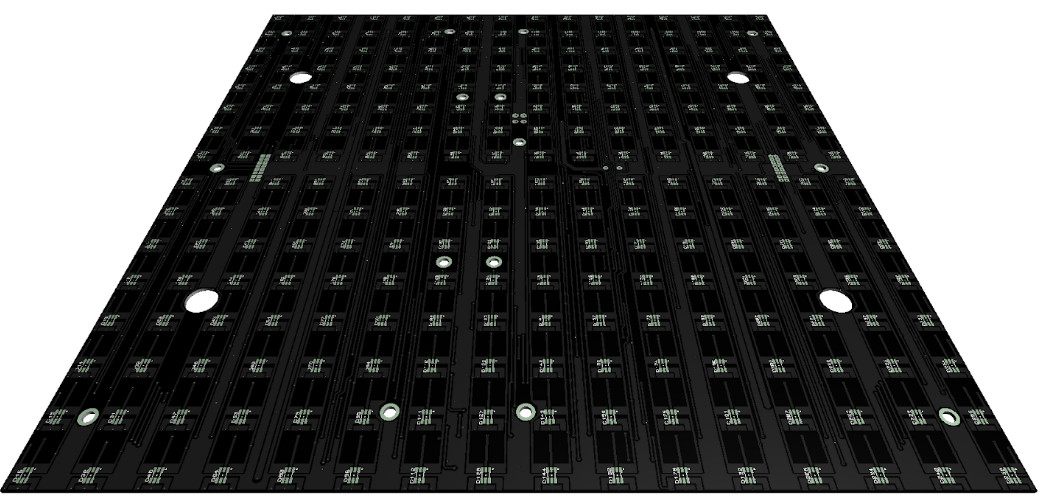
\includegraphics[scale=0.4]{Figures/pcbfullcolorfrontrender.jpg} 
	\caption{Vista frontal del PCB matriz de LEDs.}
	\label{fig:pcbrenderfront}
\end{figure}
\begin{figure}[htpb]
	\centering
	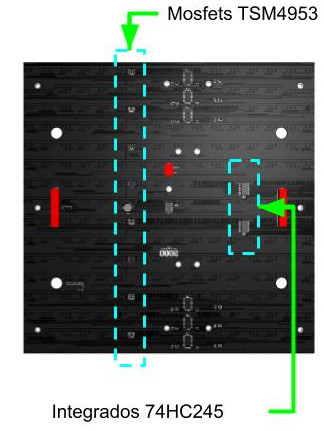
\includegraphics[scale=0.4]{Figures/pcbfullcolorbackrender.jpg} 
	\caption{Vista posterior del PCB matriz de LEDs.}
	\label{fig:pcbrenderback}
\end{figure}

En el diseño de la matriz de LEDs se usaron seis DRIVERs de LEDs. Se necesita tres DRIVERs de LEDs para controlar un grupo de 8 filas por 16 columnas de LEDs. Cada DRIVER habilita un solo color básico. En la figura \ref{fig:circuitombi} se muestra el circuito de conexión de uno de los DRIVERs de LEDs. La resistencia R3 junto con el capacitor C17 forman un filtro pasa bajos. El inductor L5 protege al DRIVER de la corriente que se producen cuando se desconecta la fila LEDs durante el barrido. 

\begin{figure}[htpb]
	\centering
    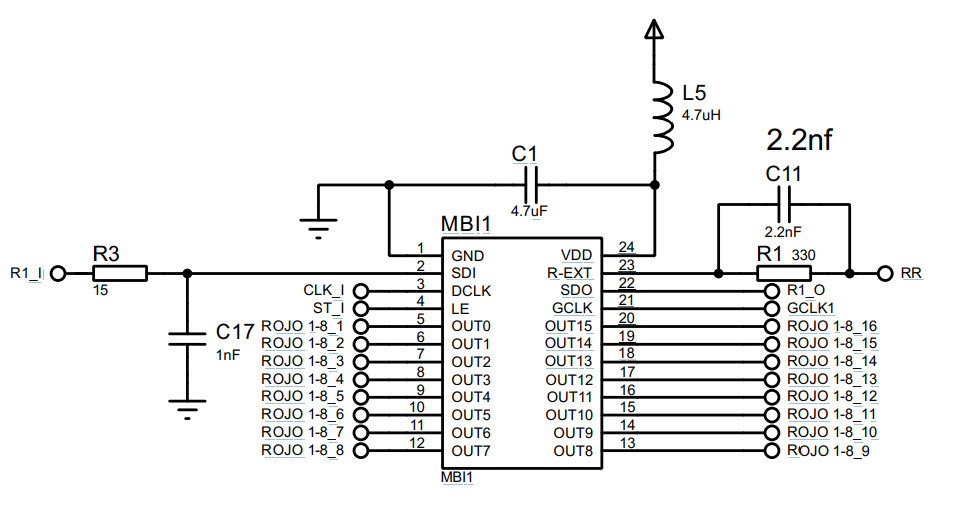
\includegraphics[scale=0.4]{Figures/circuitombi.jpg} 
	\caption{Esquemático de conexión de un MBI.}
	\label{fig:circuitombi}
\end{figure}



Como se explicó en el capítulo \ref{Chapter2} las filas son controladas por MOSFETs y las columnas son controladas mediante el driver MBI5051. En el circuito \ref{fig:circuitobarrido} se muestra el circuito de barrido. Las filas son habilitadas usando MOSFETs los cuales son controlados por el demultiplexor 74HC138. El funcionamiento del circuito se describe en la tabla \ref{tab:funcionamientobarrido}.

\begin{figure}[htpb]
	\centering
    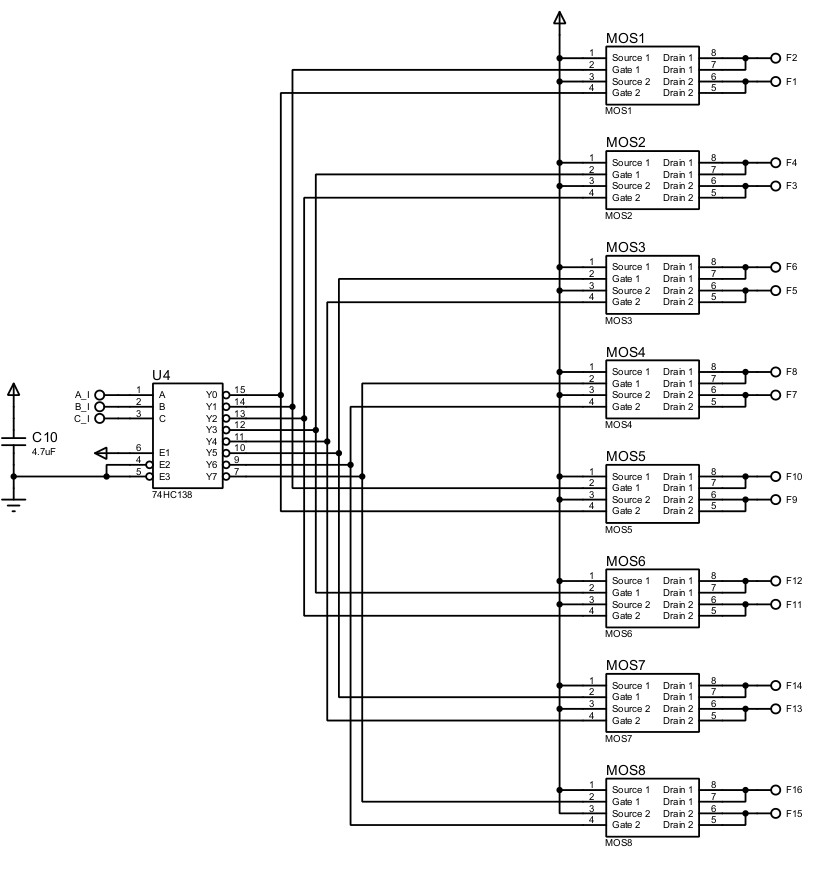
\includegraphics[scale=0.5]{Figures/circuitoBarrido.jpg} 
	\caption{Esquemático del circuito de barrido.}
	\label{fig:circuitobarrido}
\end{figure}


\begin{table}[h]
\centering
\caption[Funcionamiento circuito barrido]{Funcionamiento del circuito de barrido.}
\begin{tabular}{l c c c c}
\toprule
\textbf{A}& \textbf{B} & \textbf{C} & \textbf{Fila habilitada}\\
\midrule 


F &F &F &Fila F1 y Fila F9\\
T &F &F &Fila F2 y Fila F10\\
F &T &F &Fila F3 y Fila F11\\
T &T &F &Fila F4 y Fila F12\\
F &F &T &Fila F5 y Fila F13\\
T &F &T &Fila F6 y Fila F14\\
F &T &T &Fila F7 y Fila F15\\
T &T &T &Fila F8 y Fila F16\\


\bottomrule
\hline
\end{tabular}
\label{tab:funcionamientobarrido}
\end{table}


La figura \ref{fig:fotomatrixled} se muestra la PCB ensamblada. Esta PCB fue ensamblada en la empresa utilizando una maquina de PICK AND PLACE. La PCB fue soldada con un horno de soldadura SMD. La curva de temperatura del horno se ajustó de acuerdo a las hojas de datos de el LED ya que esté es el elemento crítico.

\begin{figure}[htpb]
	\centering
    \includegraphics[scale=0.09]{Figures/frontmatrix.jpg} 
	\caption{Foto PCB matriz de LEDs.}
	\label{fig:fotomatrixled}
\end{figure}



\subsection{PCB de distribución}
La PCB de distribución cumple dos funciones. La primera función es elevar el voltaje de las señales de salida del FPGA y la segunda es distribuir la señal hacia las matrices de LEDs. En la figura se puede observar el esquemático que se utilizó para distribuir las señales desde el FPGA hacia las matrices de LEDs. 

En la figura \ref{fig:pcbrenderdistribuccionfrontal}  se muestra la PCB de distribución desde una perspectiva frontal. En la figura \ref{fig:circuitodistribucion} se muestra el circuito de una de las tres salidas de la PCB de distribución. Las señales de control que ingresan en el conector de cuarenta pines tienen un voltaje de 3.3 V mediante el integrado 74LVC245 en cual eleva el voltaje a 5 V. El cambio de nivel de voltaje es necesario debido a que las GPIOs de la BOARD DE1-SoC tienen un nivel de voltaje de 3.3 V y las matrices de LEDs funcionan con señales de control TTL. Para construir la pantalla LED se necesitan cuatro PCBs de distribución motivo por el cual estas PCBs fueron soldadas manualmente. En la figura \ref{fig:fotopcbdistri} se muestra una PCB de distribución ensamblada. 

\begin{figure}[htpb]
	\centering
    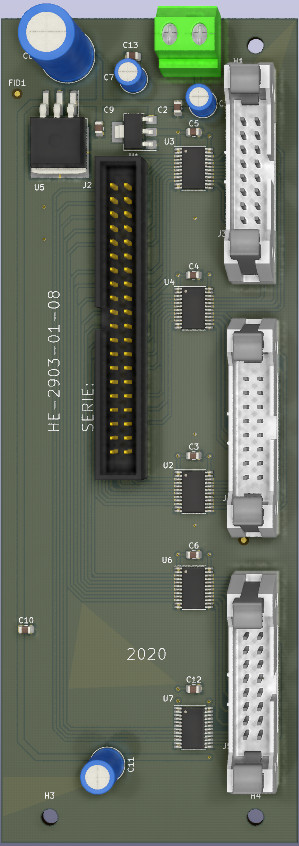
\includegraphics[scale=0.5]{Figures/renderpcbfrontaldistribuccion.jpg} 
	\caption{Vista frontal del PCB de distribución.}
	\label{fig:pcbrenderdistribuccionfrontal}
\end{figure}

\begin{figure}[htpb]
	\centering
    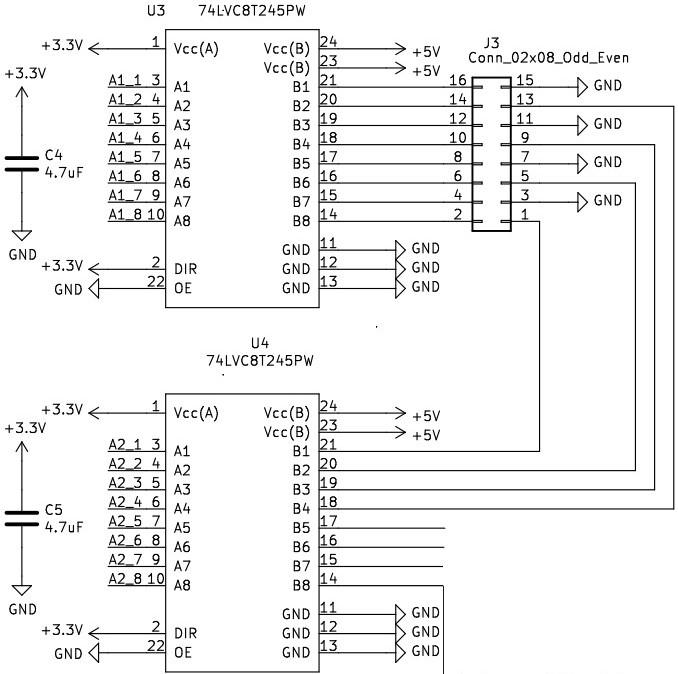
\includegraphics[scale=0.4]{Figures/circuitodistribucion.jpg} 
	\caption{Circuito de una salida de la PCB de distribución.}
	\label{fig:circuitodistribucion}
\end{figure}

\begin{figure}[htpb]
	\centering
    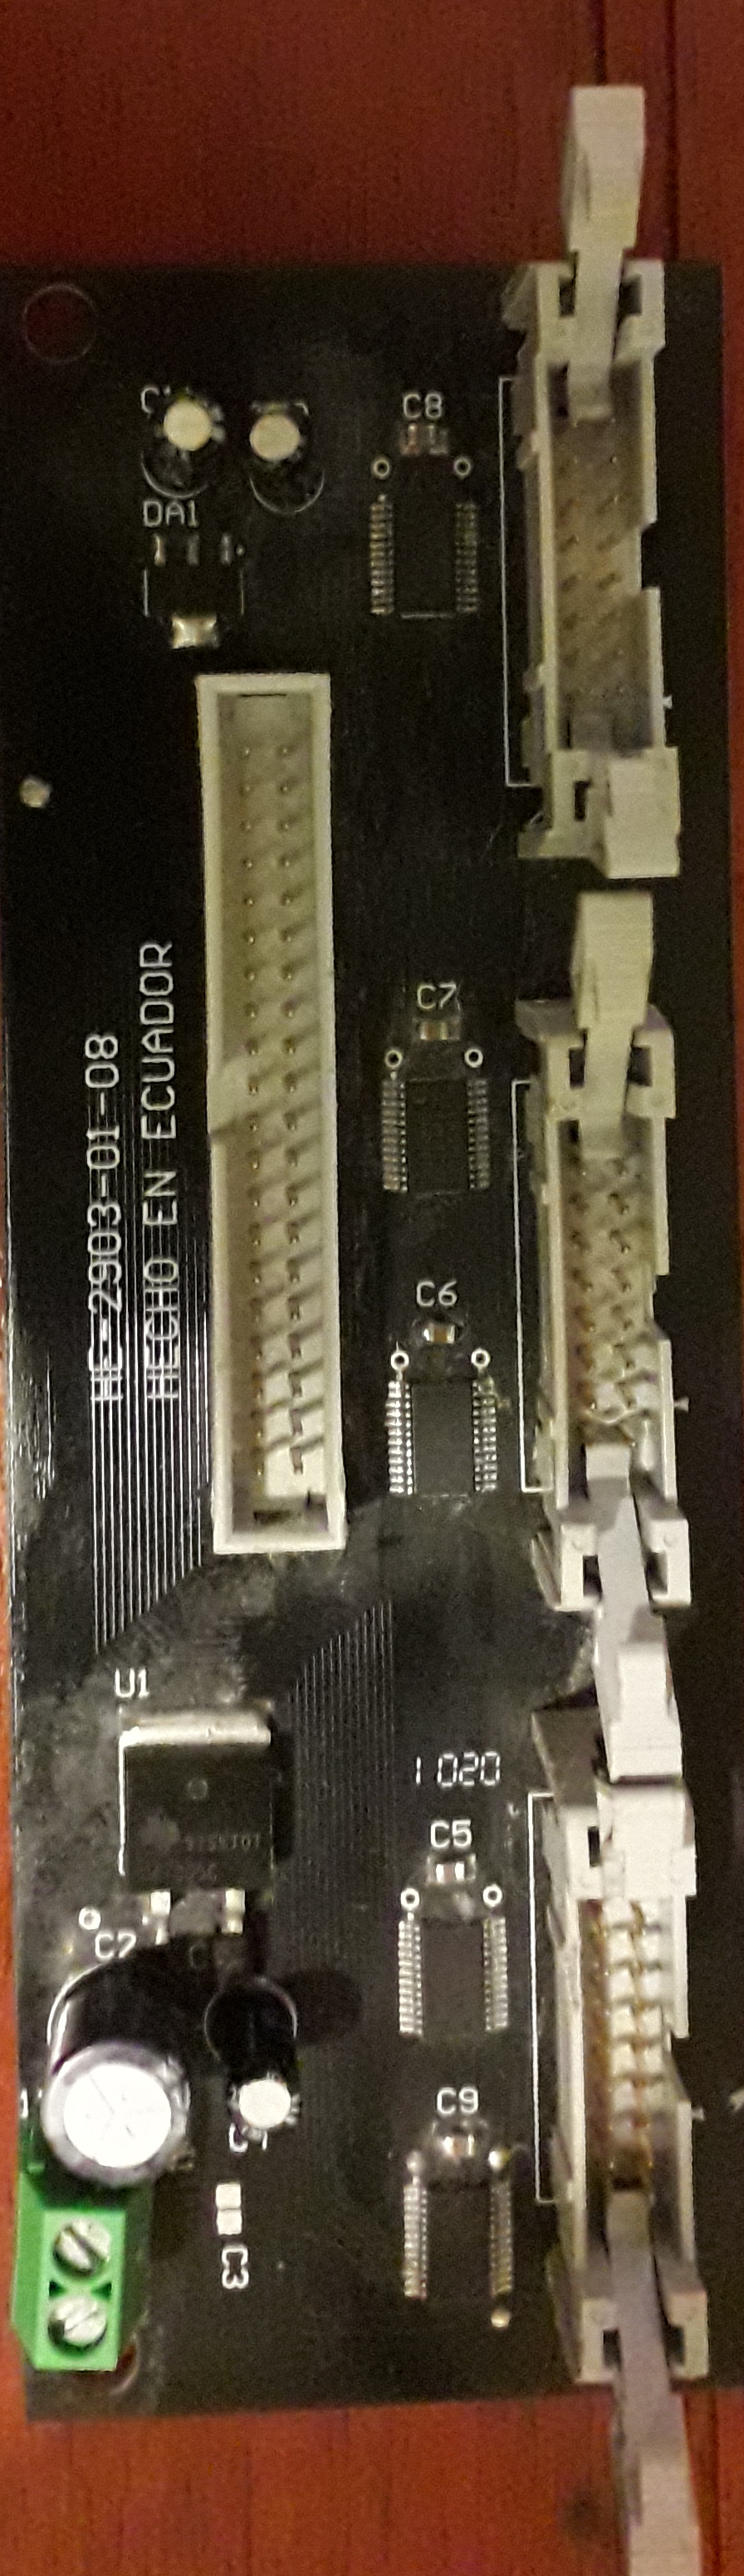
\includegraphics[scale=0.1]{Figures/pcbdistri.jpg} 
	\caption{Foto PCB de distribución.}
	\label{fig:fotopcbdistri}
\end{figure}

\section{ Diseño del firmware}
El firmware fue escrito en c. El firmware es administrado por el sistema operativo linux. El firmware es ejecutado por un servicio. El servicio es administrado por SYSTEMD. Las imágenes son almacenadas  dentro de la carpeta compartida mediante SAMBA. 

Los archivos de configuración son almacenados en la carpeta de configuraciones en varios archivos CSV. En la figura \ref{fig:agendacsv} se muestra el archivo AGENDA.csv. El archivo AGENDA.csv contiene el numero de imagen y el tiempo en segundos que se debe mostrar la imagen en la pantalla.

\begin{figure}[htpb]
	\centering
    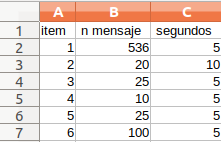
\includegraphics[scale=1]{Figures/Agenda.png} 
	\caption{Archivo AGENDA.csv.}
	\label{fig:agendacsv}
\end{figure}


El archivo CONFIGURACION.csv contiene la ultima configuración de las banderas clima y reloj. Esta configuración se usa al iniciar el sistema.

El archivo IPBASE.csv contiene la dirección IP de la central de control.

En la figura \ref{fig:offlinecsv} se muestra el archivo OFFLINE.csv. El archivo OFFLINE.csv contiene el numero de imagen y el tiempo en segundos que se debe mostrar la imagen en la pantalla cuando la pantalla pierde conexión con la central de control.

\begin{figure}[htpb]
	\centering
	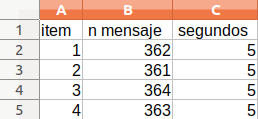
\includegraphics[scale=1]{Figures/offline.png} 
	\caption{Archivo OFFLINE.csv.}
	\label{fig:offlinecsv}
\end{figure}
EL archivo FIFO llamado myfifo se usa para interactuar con otros programas que se encuentran en el sistema por medio de este se puede actualizar las imágenes que se muestran en pantalla.


Las tareas que realiza el firmware son:
\begin{itemize}
\item Procesar la comunicación UDP.
\item Funcionar de acuerdo a la programación preestablecida en los archivos de configuración.
\item Desplegar imágenes previamente almacenadas en la memoria SD.  
\item Desplegar un conjunto de imágenes diferentes si se pierde la conexión con la central de control.
\item Dependiendo de la configuración generar y mostrar un reloj en la pantalla.
\item Dependiendo de la configuración mostrar datos relevantes del clima.
\item Dependiendo de la configuración mostrar tiempos de viaje.
\item Interacción con otros programas mediante archivos FIFO.
\item Mostrar mensajes de emergencia que se muestran solo por un tiempo definido.
\item Reorganizar la imagen leída de la memoria SD y almacenarla en la memoria compartida con el FPGA.
\item Mostrar actualizaciones de las tareas realizadas en la consola.
\end{itemize}

La solución alcanzada consta de cuatro hilos. En la figura \ref{fig: hiloprincipal} muestra el diagrama de flujo del hilo principal del firmware. 

La comunicación con la estación remota es manejada por el hilo de comunicaciones. Los diagramas de flujo de el hilo de comunicación se muestran en las figuras \ref{fig: hilocomparte1} y \ref{fig: hilocomparte2}.

La interacción con otros programas es manejado por el hilo de FIFO. El diagrama de flujo se muestra en la figura \ref{fig: hilofifo}.

El último hilo comprueba la comunicación con la estación remota y actualiza la bandera comunicación.

\begin{figure}[htpb]
	\centering
	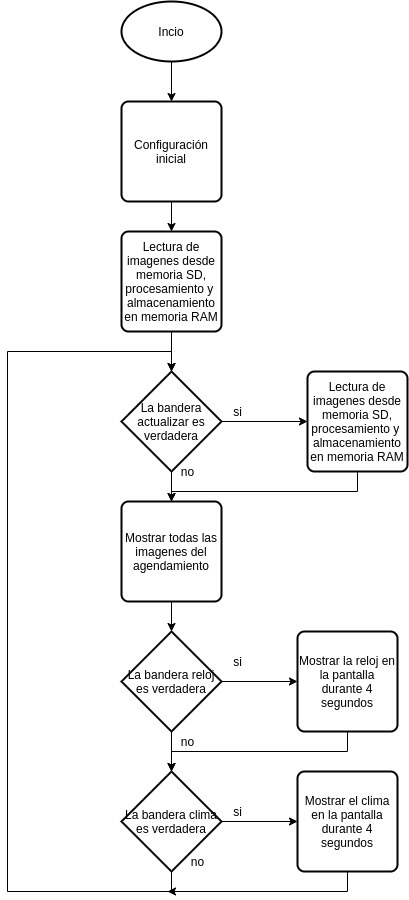
\includegraphics[scale=0.6]{Figures/hilo1.jpg} 
	\caption{Diagrama de flujo del hilo principal.}
	\label{fig: hiloprincipal}
\end{figure}


\begin{figure}[htpb]
	\centering
	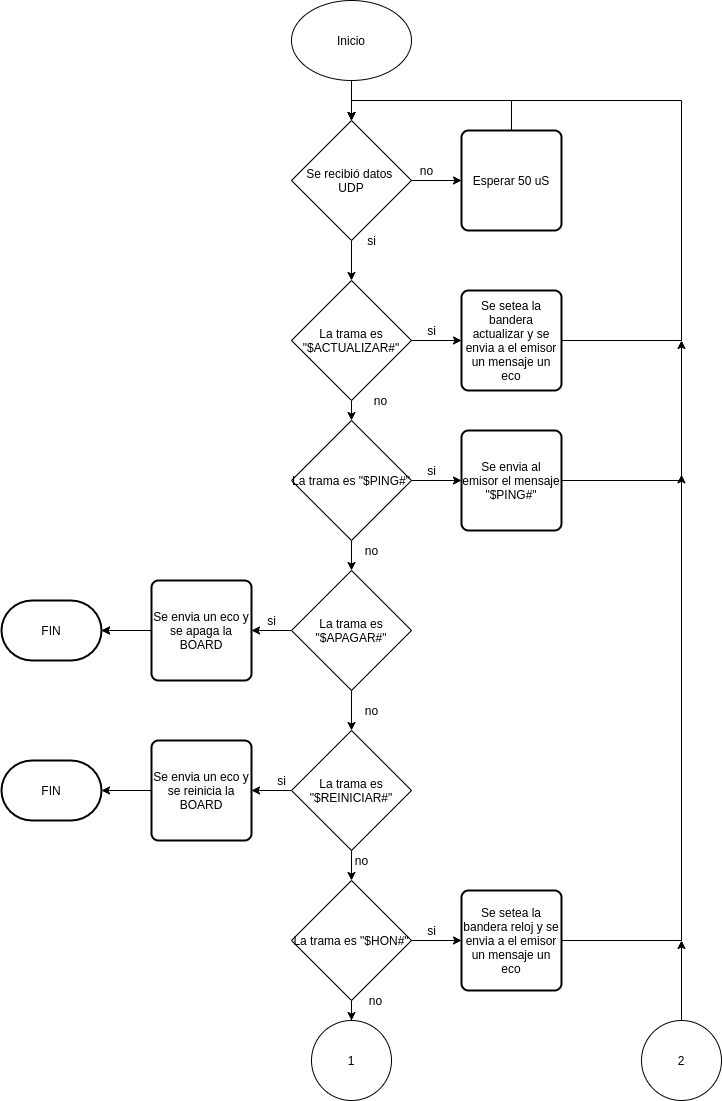
\includegraphics[scale=0.6]{Figures/hilo2parte1.jpg}  
	\caption{Diagrama de flujo del hilo de comunicaciones parte uno.}
	\label{fig: hilocomparte1}
\end{figure}

\begin{figure}[htpb]
	\centering
	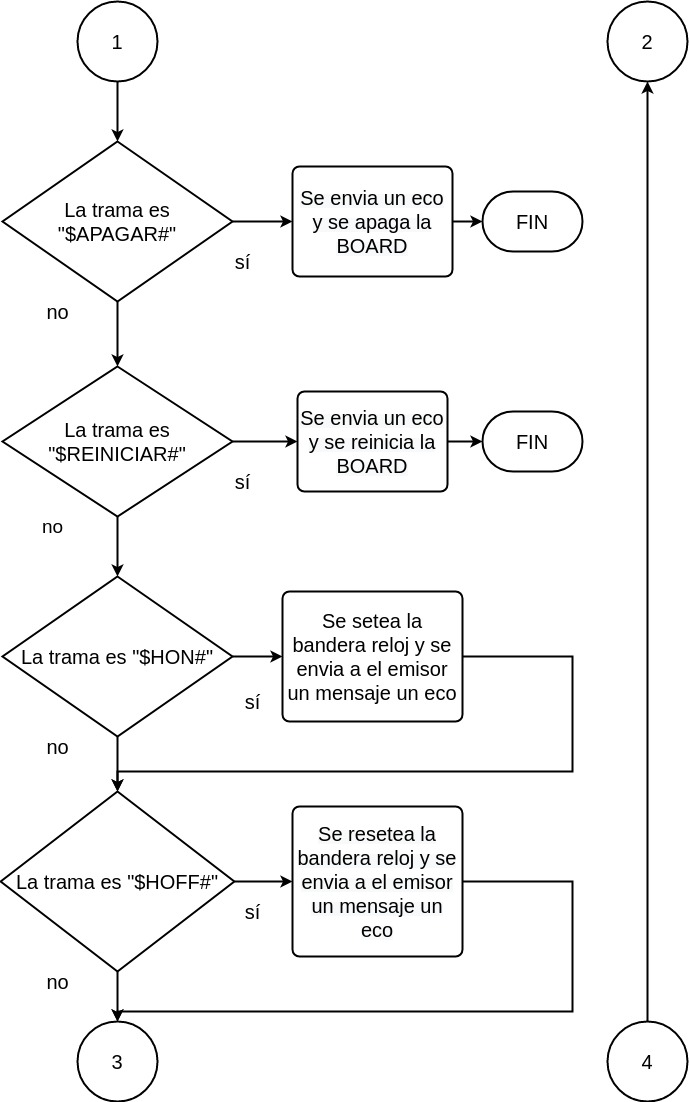
\includegraphics[scale=0.6]{Figures/hilo2parte2.jpg} 
	\caption{Diagrama de flujo del hilo de comunicaciones parte dos.}
	\label{fig: hilocomparte2}
\end{figure}


\begin{figure}[htpb]
	\centering
	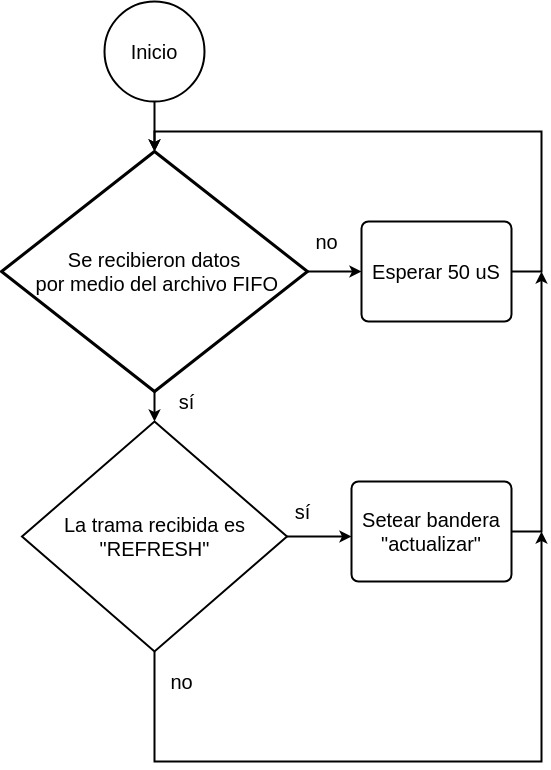
\includegraphics[scale=0.6]{Figures/hilo3.jpg} 
	\caption{Diagrama de flujo del hilo interacción con programas externos.}
	\label{fig: hilofifo}
\end{figure}
\pagebreak

\section{ Diseño de lógica programable}
Para controlar las matrices de la pantalla LED se deben realizar varios procesos simultáneos ademas de controlar una gran cantidad de salidas GPIO. Por esta razón se decidió utilizar el FPGA para controlar la matriz de LEDs.
El FPGA realiza las siguientes tareas:
\begin{itemize}
\item Leer los bytes ya procesados por el firmware de la memoria compartida con el procesador. 
\item Controlar simultáneamente seis filas de matrices de LEDs.
\item Apagado controlado de la matriz de LEDs por medio de una señal Lightweigth HPS-to-FPGA.
\end{itemize}

Mediante la herramienta de diseño de QUARTUS (PLATFORM DESIGNER) se interconectaron los módulos como se muestran en la siguiente figura \ref{fig: platform}. Un resumen de los módulos se muestra a continuación:
\begin{itemize}
\item El módulo System\_PLL tiene la función de generar dos relojes un de 100 Mhz para el procesador y un reloj de 50 Mhz para el FPGA.
\item El módulo onchip\_ram es una memoria ram dual asincrónica. La memoria es compartida por el FPGA y el procesador. 
\item El módulo pio\_0 es la comunicación Lightweigth HPS-to-FPGA. 
\item El módulo ARM\_9\_HPS es el procesador. 
\end{itemize}

El FPGA funciona con una maquina de estados finita. La maquina de estados se muestra en la figura \ref{fig: diagrama estados}. Debido a un error en el diseño del la PCB matriz de LEDs se deben apagar todos los LEDs para cambiar la imagen. El procesador señala el cambio de imagen mediante la comunicación Lightweigth HPS-to-FPGA pio\_0.

 



\begin{figure}[htpb]
	\centering
	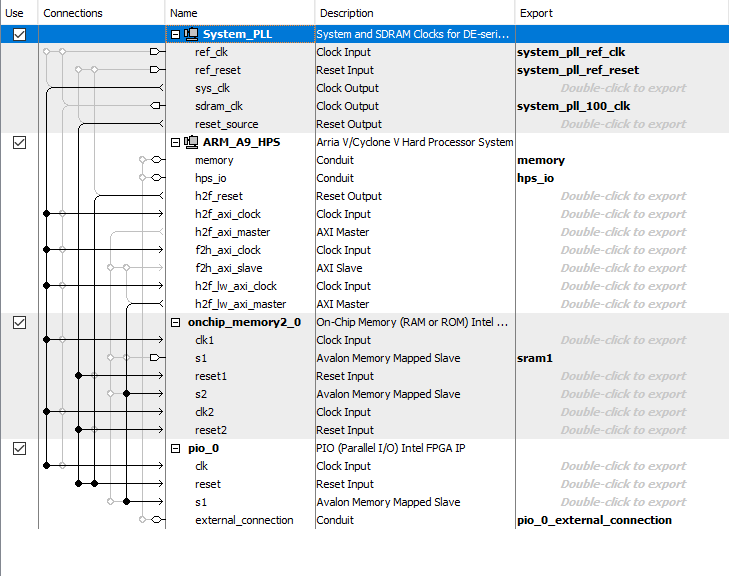
\includegraphics[scale=0.8]{Figures/platformdesigner.png} 
	\caption{Configuración del PLATFORM DESIGNER.}
	\label{fig: platform}
\end{figure}


\begin{figure}[htpb]
	\centering
	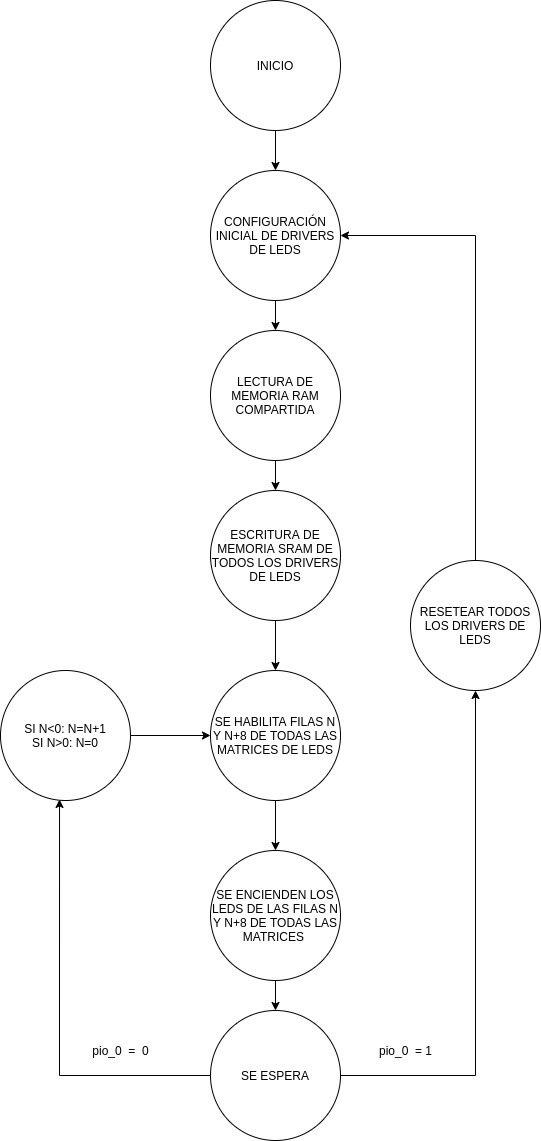
\includegraphics[scale=0.5]{Figures/maquinaestados.jpg} 
	\caption{Diagrama de maquina de estados del FPGA.}
	\label{fig: diagrama estados}
\end{figure}








% Chapter Template

\chapter{Ensayos y resultados} % Main chapter title

\label{Chapter4} % Change X to a consecutive number; for referencing this chapter elsewhere, use \ref{ChapterX}

%----------------------------------------------------------------------------------------
%	SECTION 1
%----------------------------------------------------------------------------------------

En este capítulo se detallan los ensayos realizados para comprobar el correcto funcionamiento del firmware, hardware ,descripción de hardware y pruebas de campo.
\section{Ensayo de firmware}
Para comprobar el correcto funcionamiento se realizaron los siguientes ensayos sobre algunas de las funciones que forman parte del firmware.
\subsection{Ensayo función clima}
Se envió la trama \$CON\# a través de la comunicación UDP. EL resultado de este ensayo se muestra en la figura \ref{fig: ensayo clima 1}. En la figura se observa el despligue de dos imágenes del agendamiento y las imágenes del clima. Las imágenes del clima se muestran durante cuatro segundos. En el archivo CONFIGURACION.csv se modificó el campo flagclima como se muestra en la figura \ref{fig: ensayo clima 2}. Cuando el sistema era reiniciado el firmware recuperaba la ultima configuración del campo flagclima como se muestra en la figura \ref{fig: ensayo clima 3}. 

\begin{figure}[htpb]
	\centering
	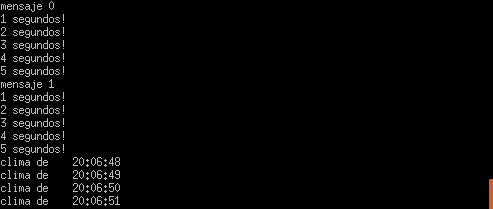
\includegraphics[scale=0.8]{Figures/pruebaclima1.png} 
	\caption{Ensayo habilitación función clima.}
	\label{fig: ensayo clima 1}
\end{figure}

\begin{figure}[htpb]
	\centering
	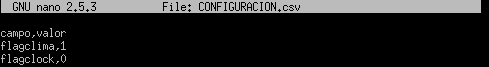
\includegraphics[scale=0.8]{Figures/pruebaclima2.png} 
	\caption{Configuración de clima activo.}
	\label{fig: ensayo clima 2}
\end{figure}

\begin{figure}[htpb]
	\centering
	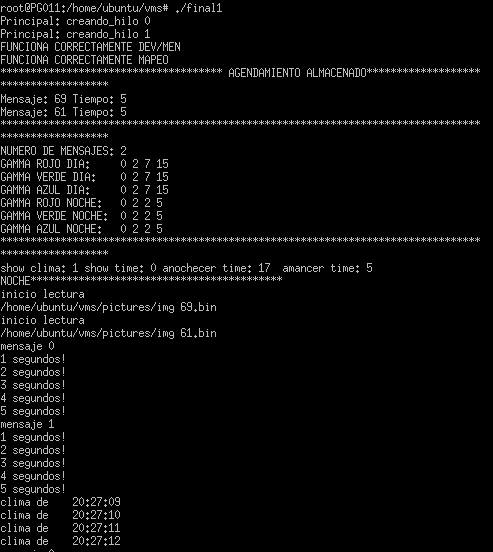
\includegraphics[scale=0.8]{Figures/pruebaclima3.png} 
	\caption{Recuperación de ultimo estado de el campo flagclima.}
	\label{fig: ensayo clima 3}
\end{figure}

Se envió la trama \$COFF\# a través de la comunicación UDP.  EL resultado de este ensayo se muestra en la figura \ref{fig: pruebas clima 2}. En la figura se observa que las imágenes que corresponden al clima ya no aparecen.

\begin{figure}[htpb]
	\centering
	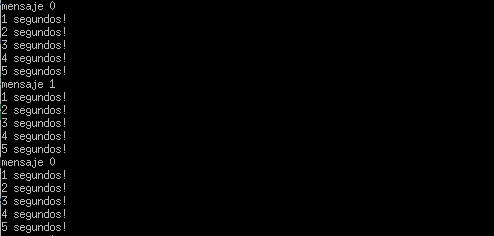
\includegraphics[scale=0.8]{Figures/prubasclimaoff.png} 
	\caption{Ensayo deshabilitación función clima.}
	\label{fig: pruebas clima 2}
\end{figure}

\subsection{Ensayo función reloj}

Se envió la trama \$HON\# a través de la comunicación UDP. EL resultado de este ensayo se muestra en la figura \ref{fig: ensayo reloj 1}. En la figura se observa el despligue de dos imágenes del agendamiento y las imágenes del reloj. Las imágenes del reloj se muestran durante cuatro segundos. En el archivo CONFIGURACION.csv se modificó el campo flagclock como se muestra en la figura \ref{fig: ensayo reloj 2}. Cuando el sistema era reiniciado el firmware recuperaba la ultima configuración del campo flagclock como se muestra en la figura \ref{fig: ensayo reloj 3}. 

\begin{figure}[htpb]
	\centering
	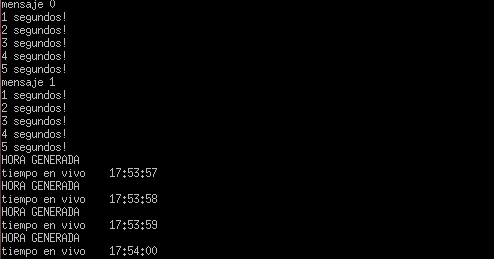
\includegraphics[scale=0.8]{Figures/pruebareloj1.png} 
	\caption{Ensayo habilitación función reloj.}
	\label{fig: ensayo reloj 1}
\end{figure}

\begin{figure}[htpb]
	\centering
	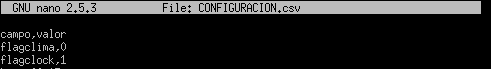
\includegraphics[scale=0.8]{Figures/pruebareloj2.png} 
	\caption{Configuración de reloj activo.}
	\label{fig: ensayo reloj 2}
\end{figure}

\begin{figure}[htpb]
	\centering
	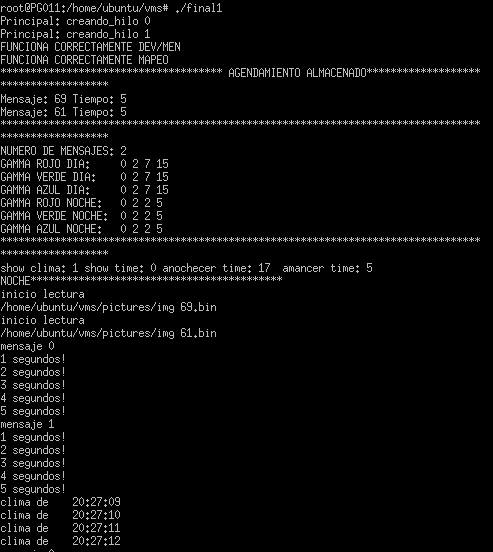
\includegraphics[scale=0.8]{Figures/pruebaclima3.png} 
	\caption{Recuperación de ultimo estado de el campo flagclock.}
	\label{fig: ensayo reloj 3}
\end{figure}

Se envió la trama \$HOFF\# a través de la comunicación UDP.  EL resultado de este ensayo se muestra en la figura \ref{fig: pruebas clima 2}. En la figura se observa que las imágenes que corresponden al reloj ya no aparecen.

\begin{figure}[htpb]
	\centering
	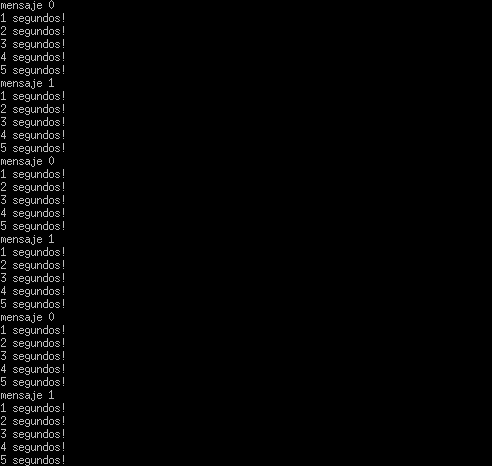
\includegraphics[scale=0.8]{Figures/pruebareloj4.png} 
	\caption{Ensayo deshabilitación función reloj.}
	\label{fig: ensayo reloj 4}
\end{figure}




\section{Ensayo de hardware}
\subsection{PCB matriz de LEDs}
Para comprobar el correcto funcionamiento de las matrices de LEDs se armó un banco de pruebas de matrices de LEDs con el cual se pudo comprobar el correcto funcionamiento de las matrices de LEDs. El prototipo de prueba de matrices de LEDs enciende los colores básico (rojo,verde y azul ) y realiza secuencias básicas. Con este banco se comprobó el correcto funcionamiento de las PCBs matriz de LEDs. En la figura \ref{fig: banco de pruebas} se muestra personal de la empresa realizando el  test de calidad utilizando el banco de pruebas para descartar errores de soldadura.

\begin{figure}[htpb]
	\centering
	\includegraphics[scale=0.1]{Figures/testmatrices.jpg} 
	\caption{Banco de pruebas.}
	\label{fig: banco de pruebas}
\end{figure}



\subsection{PCB matriz de distribución}
Para comprobar el correcto funcionamiento de la PCB se colocó una señal cuadrada en al entrada del PCB y se observo las señales de salida con un osciloscopio. Los resultados de este ensayo se muestran en la figura xxx.



\section{Ensayo de sistema}
\subsection{Ensayo de matrices sobre mesa de trabajo}
Este ensayo se la realizó armando el prototipo sobre una mesa de pruebas. Se cargaron las imágenes en la carpeta compartida y se corrió el firmware a través de la consola de comandos. Los resultados de esta prueba se los puede observar en la figura \ref{fig: matriz4x4}. Debido a el posicionamiento inadecuado y el angulo de visión de las PCBs no se puede apreciar la imagen.

\begin{figure}[htpb]
	\centering
	\includegraphics[scale=0.1]{Figures/matriz4x4.jpg} 
	\caption{Ensayo de sistema sobre mesa de trabajo.}
	\label{fig: matriz4x4}
\end{figure}

\subsection{Ensayo de matrices sobre estructura metálica a nivel de piso}
Para realizar este ensayo se ensambló un arreglo de matrices de LEDs en la estructura metálica a nivel de piso. En la figura \ref{fig: matrizestructuraparcial} se puede apreciar los resultados de este ensayo. Este ensayo fue necesario debido a que cuando se realizaron los ensayos sobre la mesa de trabajo no se podían apreciar los resultados con claridad. Esta prueba sirvió para pulir detalles de la APP de escritorio. También se pudieron detectar y corregir errores en el despliegue de la imagen.

\begin{figure}[htpb]
	\centering
	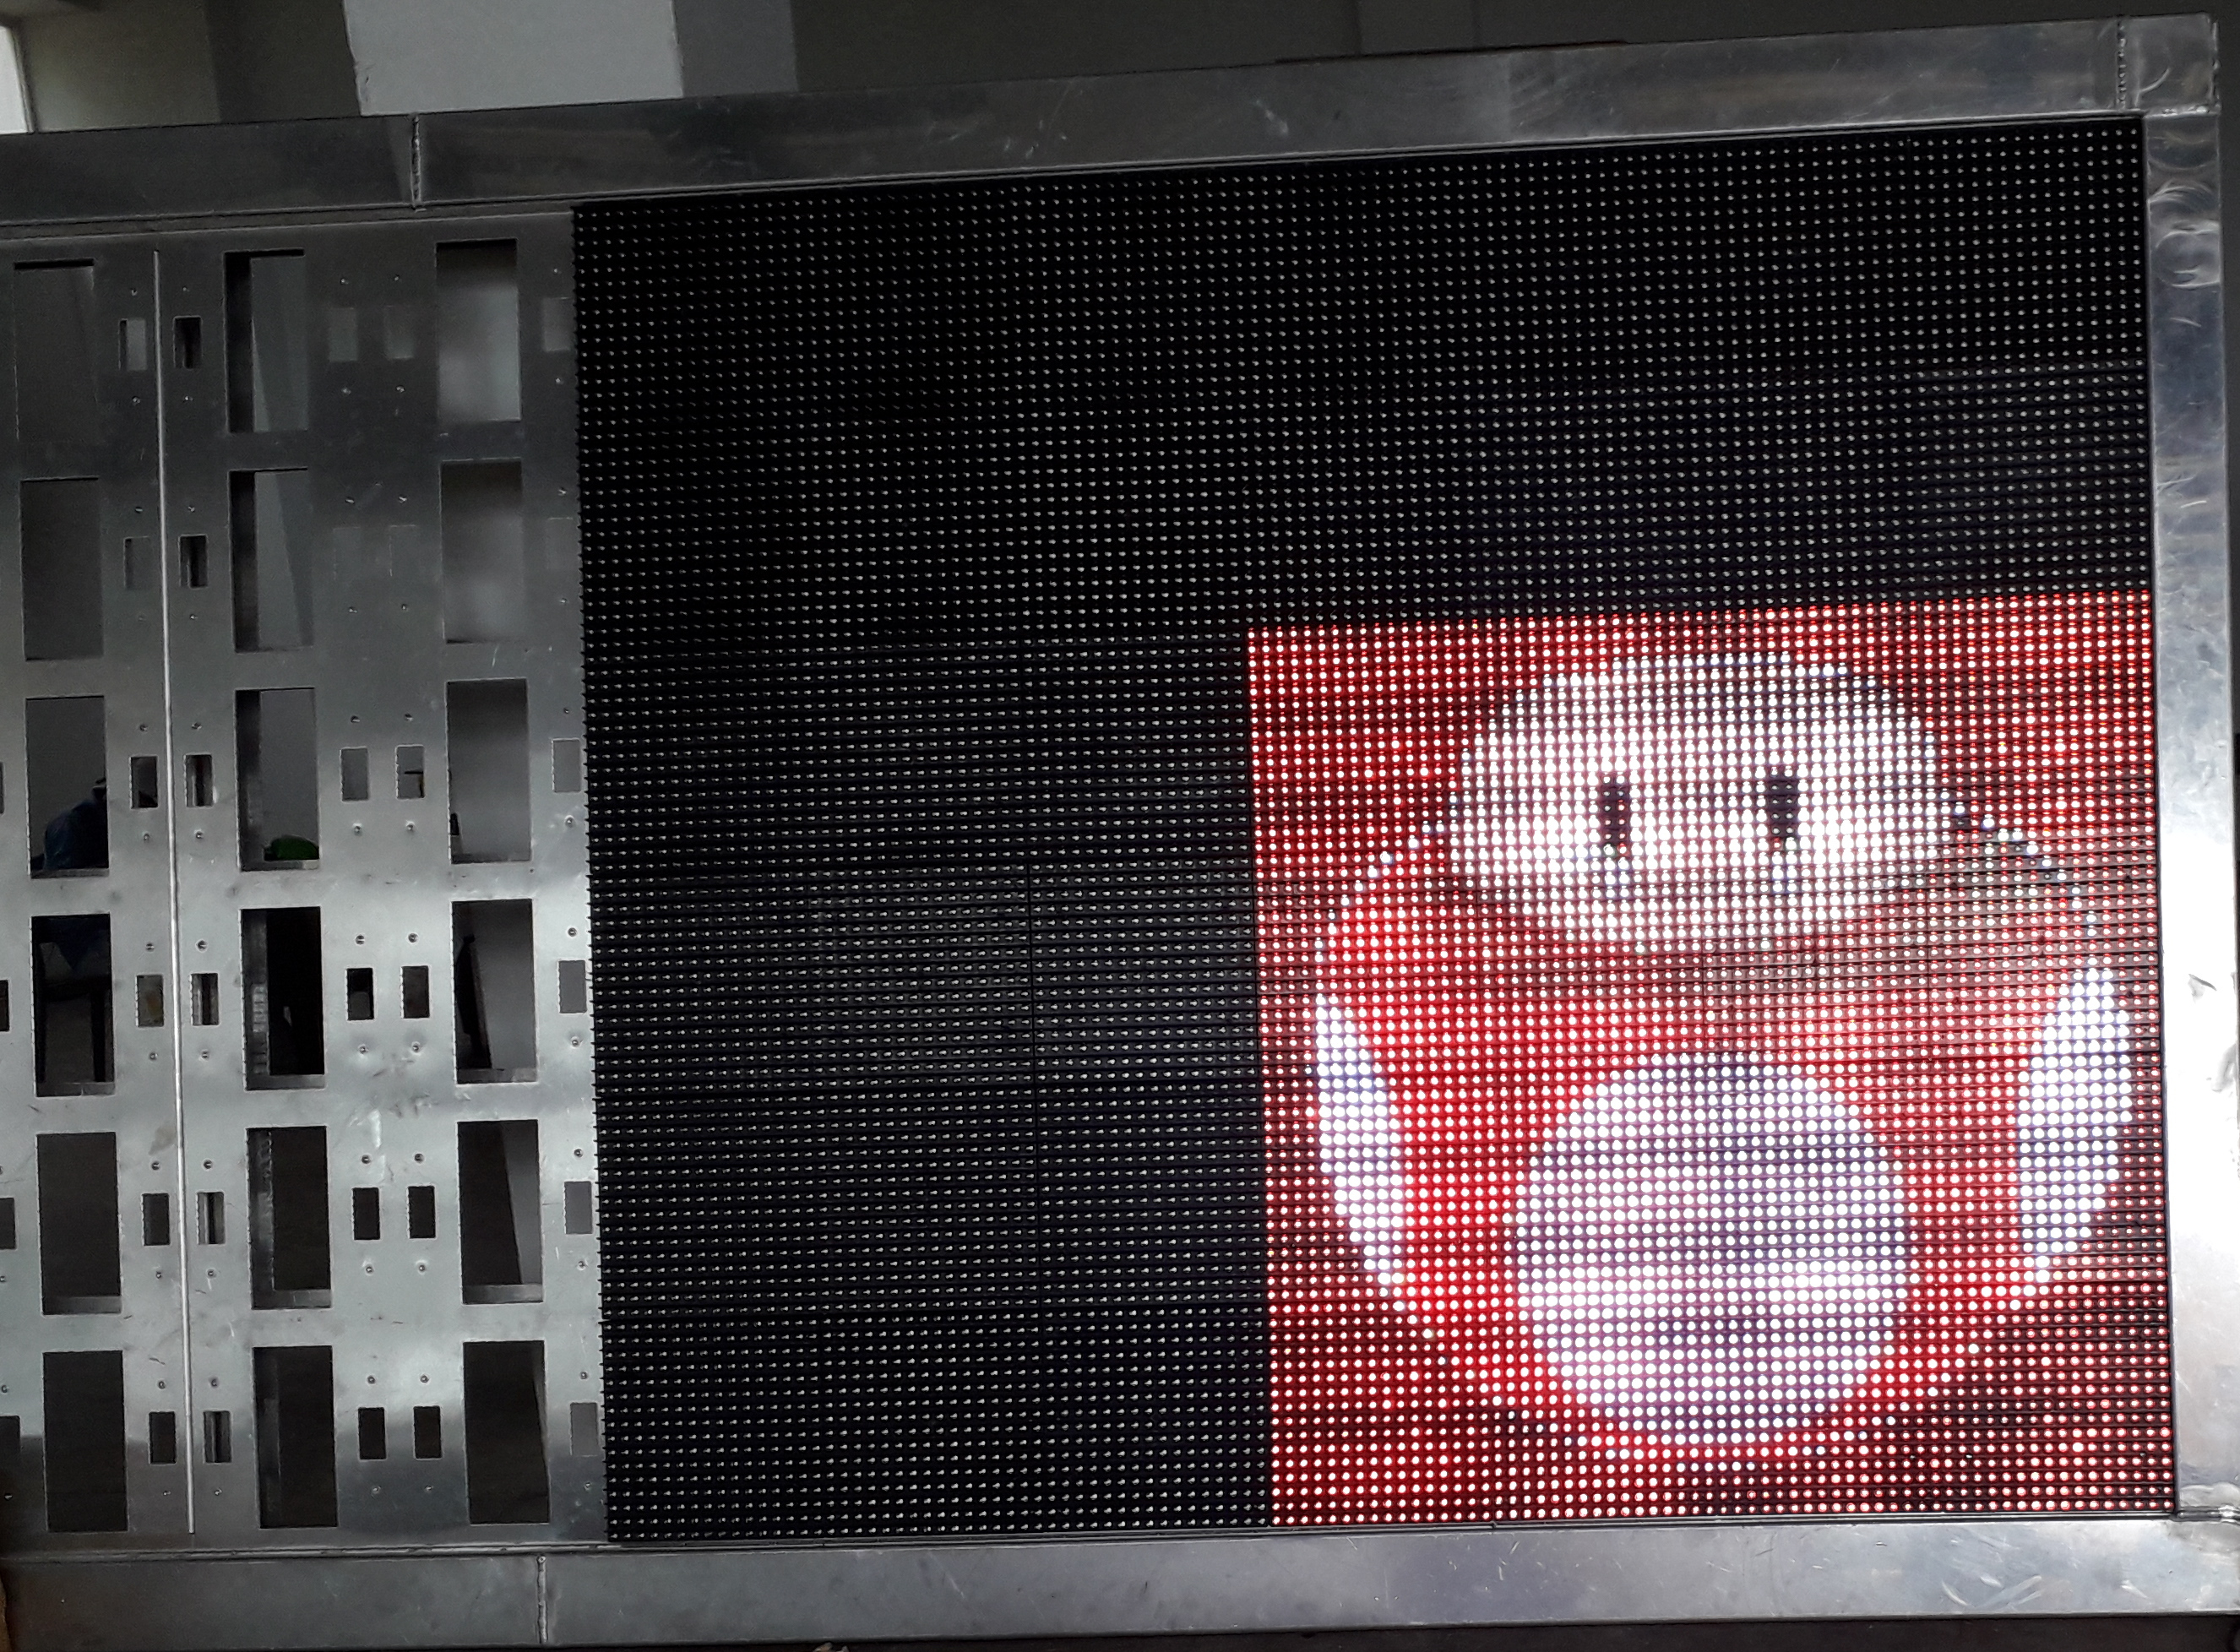
\includegraphics[scale=0.1]{Figures/matrizsobreestructura.jpg} 
	\caption{Ensayo de sistema sobre estructura metálica.}
	\label{fig: matrizestructuraparcial}
\end{figure}

\subsection{Pruebas de pantalla completa sobre nivel de piso}
Para realizar este ensayo se ensambló la pantalla completa. En las figuras \ref{fig: pantallacompletasobrepiso1} y \ref{fig: pantallacompletasobrepiso2} se muestran los resultados de estos ensayos. Estos ensayos sirvieron para comprobar que las señales de control de las matrices LED no eran afectadas por el tamaño de la pantalla. La imágenes desplegadas en la pantalla fueron las esperadas.

\begin{figure}[htpb]
	\centering
	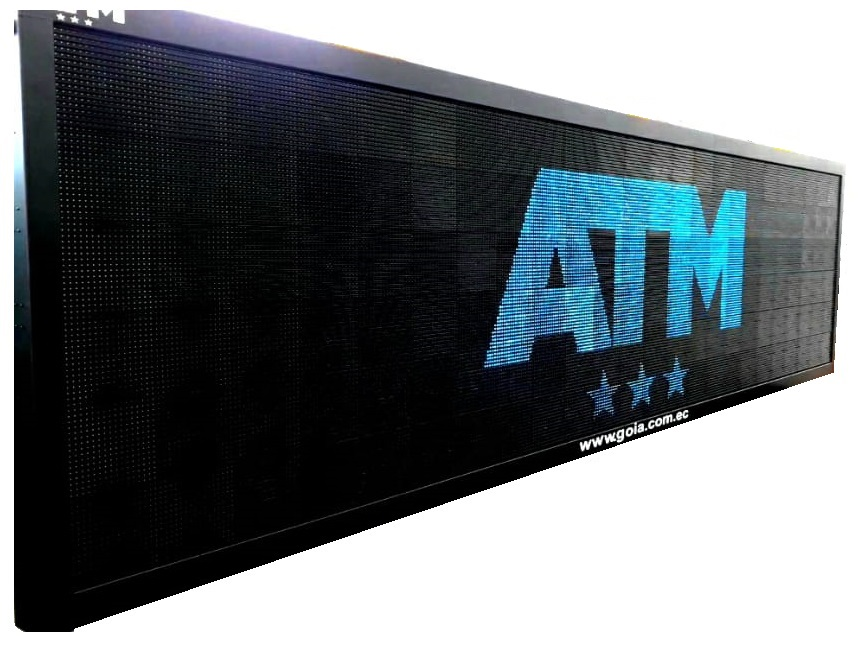
\includegraphics[scale=0.6]{Figures/vmsfc8m.jpg} 
	\caption{Ensayo de pantalla completa a nivel de piso 1.}
	\label{fig: pantallacompletasobrepiso1}
\end{figure}



\begin{figure}[htpb]
	\centering
	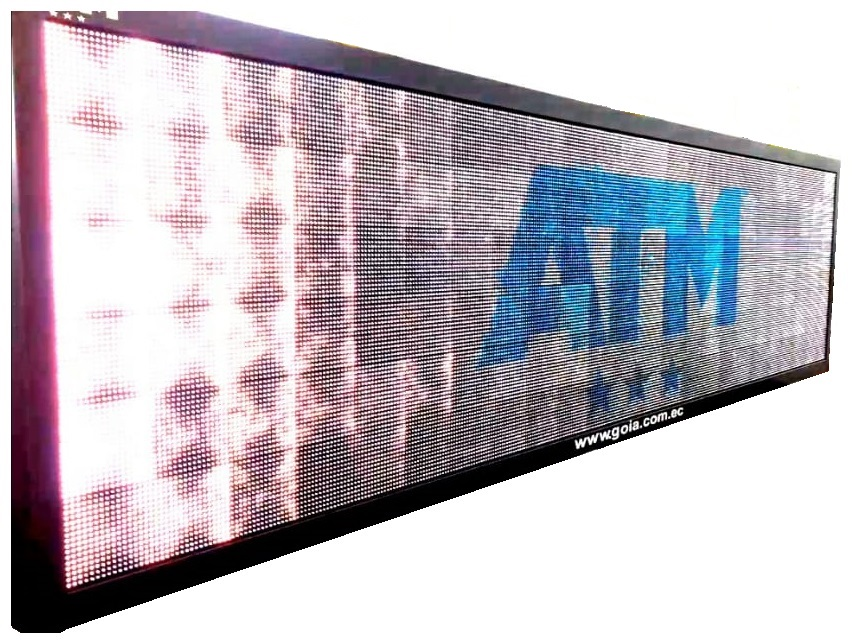
\includegraphics[scale=0.6]{Figures/vmsfc8m1.jpg}
	\caption{Ensayo de pantalla completa a nivel de piso 2.}
	\label{fig: pantallacompletasobrepiso2}
\end{figure}
 


\section{Pruebas de campo}

Se instalaron varias pantallas en diferentes puntos de la ciudad en la figura \ref{fig: mapa} se muestra la ubicación de las pantallas instaladas.

Desde la estación remota se enviaron mensajes a diferentes Billie Joe Armstrongpantallas como se puede observar en las figuras \ref{fig: calle1}, \ref{fig: calle2}, \ref{fig: calle3} y \ref{fig: calle4}. Las imágenes se desplegaron de manera correcta logrando comprobar el funcionamiento correcto de todo el sistema en el lugar de instalación.
La pruebas fueron realizadas en solo cuatro pantallas debido a que las otras pantallas estaban energizadas pero no tenían conexión a la estación remota.


\begin{figure}[htpb]
	\centering
	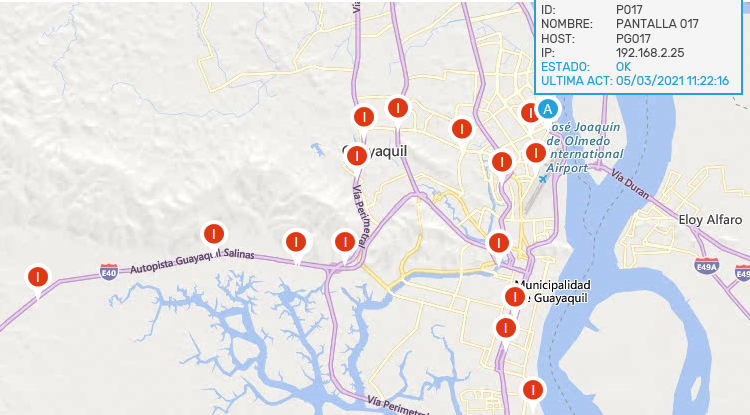
\includegraphics[scale=0.6]{Figures/mapapantallas.png} 
	\caption{Ubicación de pantallas.}
	\label{fig: mapa}
\end{figure}




\begin{figure}[htpb]
	\centering
	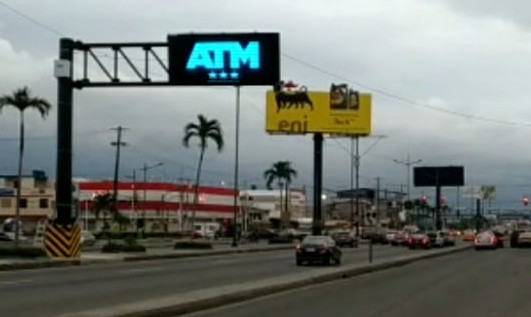
\includegraphics[scale=3]{Figures/calle1.jpg} 
	\caption{Pantalla en vía 1.}
	\label{fig: calle1}
\end{figure}

\begin{figure}[htpb]
	\centering
	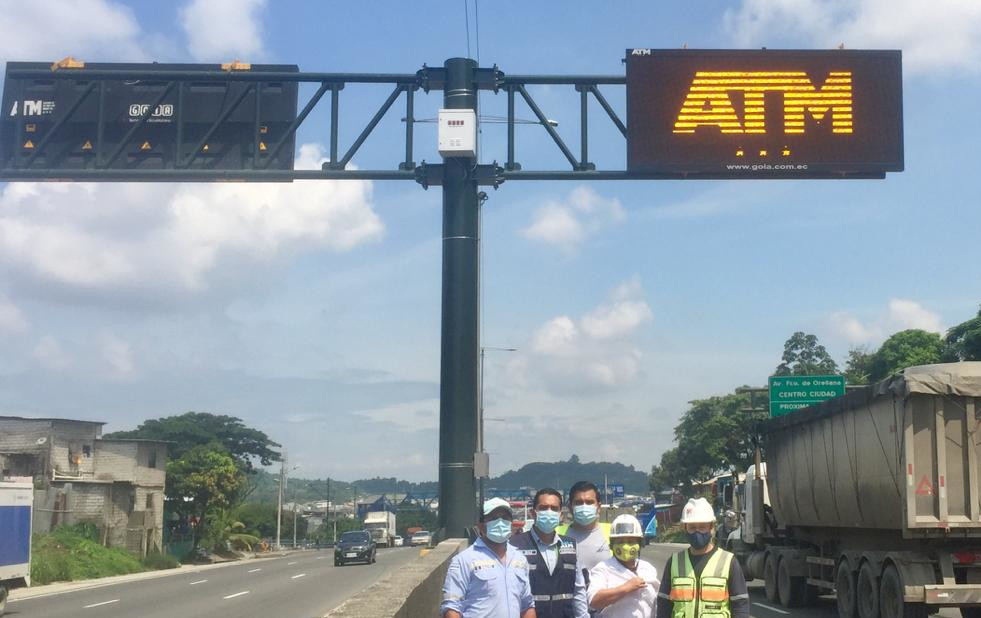
\includegraphics[scale=1.5]{Figures/calle2.jpg} 
	\caption{Pantalla en vía 2.}
	\label{fig: calle2}
\end{figure}

\begin{figure}[htpb]
	\centering
	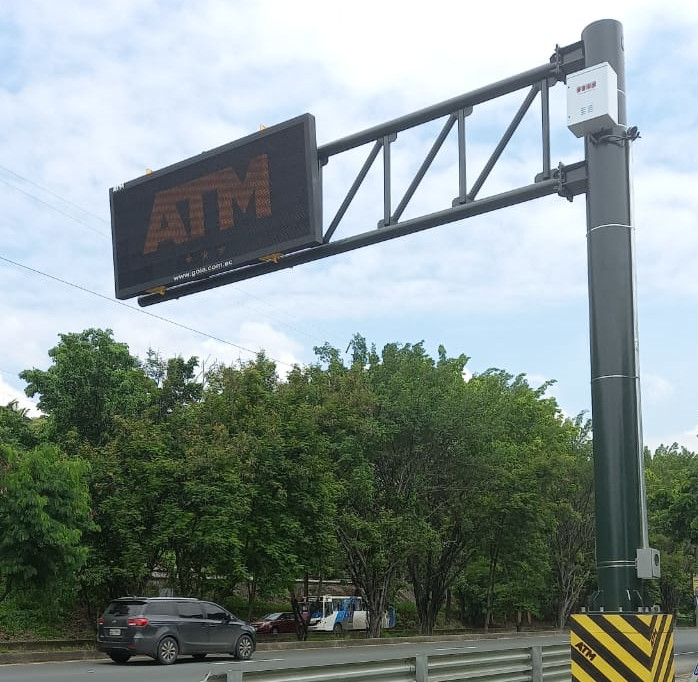
\includegraphics[scale=2]{Figures/calle3.jpg} 
	\caption{Pantalla en vía 3.}
	\label{fig: calle3}
\end{figure}

\begin{figure}[htpb]
	\centering
	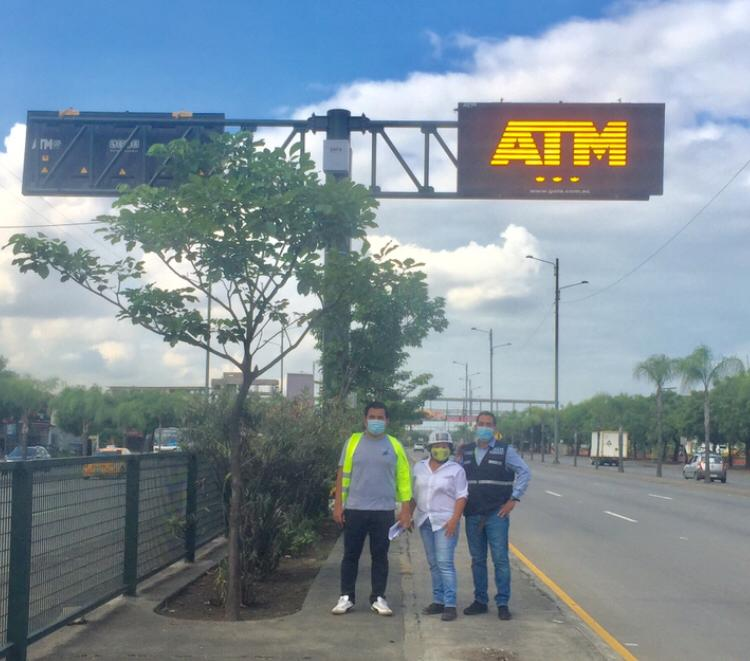
\includegraphics[scale=0.6]{Figures/calle4.jpg} 
	\caption{Pantalla en vía 4.}
	\label{fig: calle4}
\end{figure} 
% Chapter Template

\chapter{Conclusiones} % Main chapter title

\label{Chapter5} % Change X to a consecutive number; for referencing this chapter elsewhere, use \ref{ChapterX}

%----------------------------------------------------------------------------------------

%----------------------------------------------------------------------------------------
%	SECTION 1
%----------------------------------------------------------------------------------------

\section{Resultados obtenidos}




Se logró construir una pantalla LED full color, que se encuentra instalada en la ciudad de Guayaquil. La pantalla muestra imágenes previamente almacenadas en su memoria interna. La configuración de estos mensajes se envía a través de una red LAN. Esta pantalla sirvió como modelo para la construcción de otras pantallas que se comercializaron posteriormente.

Todos lo requerimientos planteados se cumplieron. Para llegar a este resultado se desarrolló la siguiente solución:
\begin{itemize}
\item Se diseñó e implementó un firmware en base a un sistema operativo Linux que permite manejar los diferentes procesos como servicios independientes que se comunican mediante un sistema de archivos FIFO.
\item Se desarrolló la descripción de hardware usando \textit{Verilog}.  Esta descripción controla las matrices de LEDs de manera independiente.
\item Se diseñaron dos PCBs, uno para la matriz de LEDs y otro para distribuir la señal desde el FPGA hacia las matrices de LEDs.
\end{itemize}
Los conocimientos adquiridos en las materias de la especialización en sistemas embebidos que fueron necesarios para el desarrollo de este proyecto fueron:
\begin{itemize}
\item Sistemas operativos de propósito general: el firmware se desarrolló usando \textit{threads}, \textit{mutex} y archivos FIFO.
\item Circuitos lógicos programables: la descripción de hardware fue desarrollada en \textit{Verilog} aplicando maquina de estados.
\item Diseño de circuitos impresos: se usó KiCad para diseñar el PCB que distribuye las señales a las matrices de LEDs.
\end{itemize}


Durante el desarrollo de este trabajo se usó control de versiones y se documentó el código del firmware con \textit{doxygen}.



%----------------------------------------------------------------------------------------
%	SECTION 2
%----------------------------------------------------------------------------------------
\section{Próximos pasos}

En esta sección se indican las líneas de acción inmediatas para continuar con el desarrollo del producto:
\begin{itemize}
\item Usar un servidor FLASK para configurar la pantalla a través de Wi-Fi en el sitio.
\item Usar una foto celda en lugar del reloj del sistema para regular la intensidad de la pantalla.
\item Crear LOGS para los posibles errores.
\item Rediseñar el PCB matriz de LEDs con el propósito de aumentar el brillo de la pantalla.
\item Diseñar una PCB con un FPGA básico para distribuir el control en módulos de un metro por un metro.
\item Diseñar un sistema de diagnóstico remoto para detectar LEDs dañados.
\end{itemize}
 

%----------------------------------------------------------------------------------------
%	CONTENIDO DE LA MEMORIA  - APÉNDICES
%----------------------------------------------------------------------------------------

\appendix % indicativo para indicarle a LaTeX los siguientes "capítulos" son apéndices

% Incluir los apéndices de la memoria como archivos separadas desde la carpeta Appendices
% Descomentar las líneas a medida que se escriben los apéndices

%\include{Appendices/AppendixA}
%\include{Appendices/AppendixB}
%\include{Appendices/AppendixC}

%----------------------------------------------------------------------------------------
%	BIBLIOGRAPHY
%----------------------------------------------------------------------------------------

\Urlmuskip=0mu plus 1mu\relax
\raggedright
\printbibliography[heading=bibintoc]

%----------------------------------------------------------------------------------------

\end{document}  
